\documentclass[a4paper]{book}
\usepackage{makeidx}
\usepackage{natbib}
\usepackage{graphicx}
\usepackage{multicol}
\usepackage{float}
\usepackage{listings}
\usepackage{color}
\usepackage{ifthen}
\usepackage[table]{xcolor}
\usepackage{textcomp}
\usepackage{alltt}
\usepackage{ifpdf}
\ifpdf
\usepackage[pdftex,
            pagebackref=true,
            colorlinks=true,
            linkcolor=blue,
            unicode
           ]{hyperref}
\else
\usepackage[ps2pdf,
            pagebackref=true,
            colorlinks=true,
            linkcolor=blue,
            unicode
           ]{hyperref}
\usepackage{pspicture}
\fi
\usepackage[utf8]{inputenc}
\usepackage{mathptmx}
\usepackage[scaled=.90]{helvet}
\usepackage{courier}
\usepackage{sectsty}
\usepackage[titles]{tocloft}
\usepackage{doxygen}
\lstset{language=C++,inputencoding=utf8,basicstyle=\footnotesize,breaklines=true,breakatwhitespace=true,tabsize=8,numbers=left }
\makeindex
\setcounter{tocdepth}{3}
\renewcommand{\footrulewidth}{0.4pt}
\renewcommand{\familydefault}{\sfdefault}
\hfuzz=15pt
\setlength{\emergencystretch}{15pt}
\hbadness=750
\tolerance=750
\begin{document}
\hypersetup{pageanchor=false,citecolor=blue}
\begin{titlepage}
\vspace*{7cm}
\begin{center}
{\Large \-Vo\-Ip \\[1ex]\large 1.\-0 }\\
\vspace*{1cm}
{\large \-Generated by Doxygen 1.7.5.1}\\
\vspace*{0.5cm}
{\small Thu Dec 22 2011 04:15:13}\\
\end{center}
\end{titlepage}
\clearemptydoublepage
\pagenumbering{roman}
\tableofcontents
\clearemptydoublepage
\pagenumbering{arabic}
\hypersetup{pageanchor=true,citecolor=blue}
\chapter{\-University of \-Plymouth \-S\-O\-F\-T336 \-Coursework by \-Sam \-Gunaratne}
\label{index}\hypertarget{index}{}\hypertarget{index_About}{}\section{\-About}\label{index_About}
\-Vo\-I\-P allows you to have real time two-\/way voice communication over a local network. \-The software has no centralized server and is entirely peer to peer driven. 
\chapter{\-Class \-Index}
\section{\-Class \-Hierarchy}
\-This inheritance list is sorted roughly, but not completely, alphabetically\-:\begin{DoxyCompactList}
\item \contentsline{section}{\-Abstract\-Voice}{\pageref{class_abstract_voice}}{}
\begin{DoxyCompactList}
\item \contentsline{section}{\-Voice\-Input}{\pageref{class_voice_input}}{}
\item \contentsline{section}{\-Voice\-Output}{\pageref{class_voice_output}}{}
\end{DoxyCompactList}
\item \contentsline{section}{\-Command\-Client}{\pageref{class_command_client}}{}
\item \contentsline{section}{\-Command\-Server}{\pageref{class_command_server}}{}
\item \contentsline{section}{\-Main\-Window}{\pageref{class_main_window}}{}
\item \contentsline{section}{\-Network\-Discover}{\pageref{class_network_discover}}{}
\item \contentsline{section}{\-Peer}{\pageref{class_peer}}{}
\item \contentsline{section}{\-Receive\-Thread}{\pageref{class_receive_thread}}{}
\item \contentsline{section}{\-Send\-Thread}{\pageref{class_send_thread}}{}
\item \contentsline{section}{\-Sound\-Reciever}{\pageref{class_sound_reciever}}{}
\item \contentsline{section}{\-Sound\-Sender}{\pageref{class_sound_sender}}{}
\item \contentsline{section}{\-State\-Controller}{\pageref{class_state_controller}}{}
\end{DoxyCompactList}

\chapter{\-Class \-Index}
\section{\-Class \-List}
\-Here are the classes, structs, unions and interfaces with brief descriptions\-:\begin{DoxyCompactList}
\item\contentsline{section}{\hyperlink{class_abstract_voice}{\-Abstract\-Voice} \\*\-Abstracted common voice elements for recording and playback }{\pageref{class_abstract_voice}}{}
\item\contentsline{section}{\hyperlink{class_command_client}{\-Command\-Client} \\*\-A subclass of \-Q\-Tcp\-Socket, class that is responsible for sending/receiving control signals between callers over the network }{\pageref{class_command_client}}{}
\item\contentsline{section}{\hyperlink{class_command_server}{\-Command\-Server} \\*\-A subclass of \-Q\-Tcp\-Server that receives command signals from clients over the network }{\pageref{class_command_server}}{}
\item\contentsline{section}{\hyperlink{class_main_window}{\-Main\-Window} \\*\-Graphical interface class of type \-Q\-Main\-Window }{\pageref{class_main_window}}{}
\item\contentsline{section}{\hyperlink{class_network_discover}{\-Network\-Discover} \\*\-Discovers local peers on the network to communicate with }{\pageref{class_network_discover}}{}
\item\contentsline{section}{\hyperlink{class_peer}{\-Peer} \\*\-Holds information for a located communication peer on the network }{\pageref{class_peer}}{}
\item\contentsline{section}{\hyperlink{class_receive_thread}{\-Receive\-Thread} \\*\-A \-Thread class that controls listening for incoming voice data }{\pageref{class_receive_thread}}{}
\item\contentsline{section}{\hyperlink{class_send_thread}{\-Send\-Thread} \\*\-A \-Thread class that controls recording audio and sending data communication }{\pageref{class_send_thread}}{}
\item\contentsline{section}{\hyperlink{class_sound_reciever}{\-Sound\-Reciever} \\*\-A buffer that receives \-U\-D\-P audio data over the network }{\pageref{class_sound_reciever}}{}
\item\contentsline{section}{\hyperlink{class_sound_sender}{\-Sound\-Sender} \\*\-A buffer that sends \-U\-D\-P audio data over the network }{\pageref{class_sound_sender}}{}
\item\contentsline{section}{\hyperlink{class_state_controller}{\-State\-Controller} \\*\-This controller object contains state information and acts as a go between the view and model }{\pageref{class_state_controller}}{}
\item\contentsline{section}{\hyperlink{class_voice_input}{\-Voice\-Input} \\*\-Captures audio data and puts it in a buffer for sending down the network }{\pageref{class_voice_input}}{}
\item\contentsline{section}{\hyperlink{class_voice_output}{\-Voice\-Output} \\*\-Receives audio data and plays it using the systems default output device }{\pageref{class_voice_output}}{}
\end{DoxyCompactList}

\chapter{\-Class \-Documentation}
\hypertarget{class_abstract_voice}{
\section{\-Abstract\-Voice \-Class \-Reference}
\label{class_abstract_voice}\index{\-Abstract\-Voice@{\-Abstract\-Voice}}
}


\-Abstracted common voice elements for recording and playback.  




{\ttfamily \#include $<$abstractvoice.\-h$>$}

\-Inheritance diagram for \-Abstract\-Voice\-:\begin{figure}[H]
\begin{center}
\leavevmode
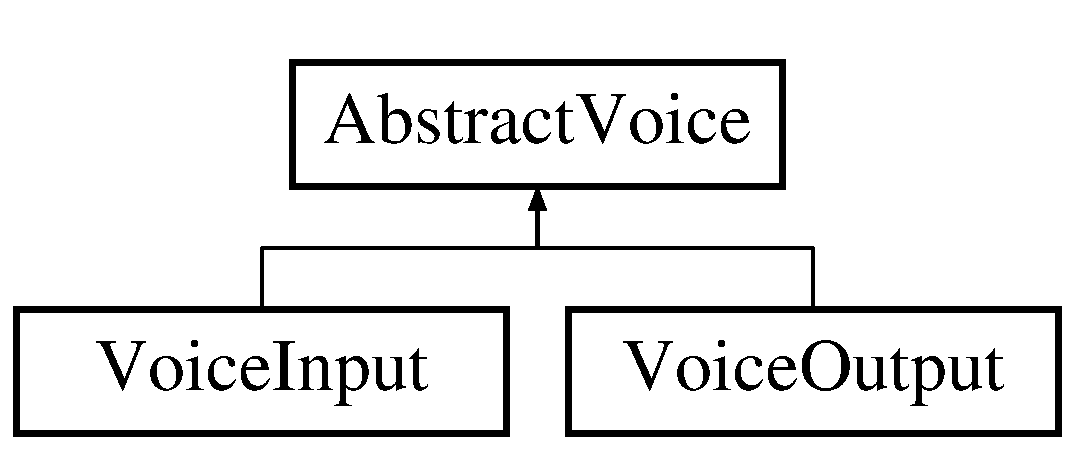
\includegraphics[height=2.000000cm]{class_abstract_voice}
\end{center}
\end{figure}
\subsection*{\-Public \-Slots}
\begin{DoxyCompactItemize}
\item 
virtual void \hyperlink{class_abstract_voice_a5e6f942915e9ef55babd7070225266ce}{start} ()=0
\begin{DoxyCompactList}\small\item\em \-A virtual function that starts the voice operation. \end{DoxyCompactList}\item 
virtual void \hyperlink{class_abstract_voice_aae2a6c918a63938881faefd9909508a0}{stop} ()=0
\begin{DoxyCompactList}\small\item\em \-A virtual function that stops all voice operation and subsequently is ready to receive another start call. \end{DoxyCompactList}\end{DoxyCompactItemize}
\subsection*{\-Public \-Member \-Functions}
\begin{DoxyCompactItemize}
\item 
\hyperlink{class_abstract_voice_a6b3c93369820d5e9e65f596dcf2147be}{\-Abstract\-Voice} (\-Q\-Object $\ast$parent=0)
\begin{DoxyCompactList}\small\item\em \-Abstract constructor. \end{DoxyCompactList}\item 
\hyperlink{class_abstract_voice_a93d6515cf6e84cad397efe6b339a1b0c}{$\sim$\-Abstract\-Voice} ()
\begin{DoxyCompactList}\small\item\em \-Abstract destructor. \end{DoxyCompactList}\end{DoxyCompactItemize}
\subsection*{\-Protected \-Attributes}
\begin{DoxyCompactItemize}
\item 
\-Q\-Audio\-Format \hyperlink{class_abstract_voice_aa8718f0af1669ef7a84347c2d9a54cf9}{format}
\begin{DoxyCompactList}\small\item\em \-Audio format to be used, default is set to audio/pcm, 8000 freq, 1 channel, 8 sample rate. \end{DoxyCompactList}\item 
\hypertarget{class_abstract_voice_ac27882c5cb69564cbc4d5cca7847a359}{
\-Q\-Audio\-Device\-Info $\ast$ \hyperlink{class_abstract_voice_ac27882c5cb69564cbc4d5cca7847a359}{dev\-Info}}
\label{class_abstract_voice_ac27882c5cb69564cbc4d5cca7847a359}

\begin{DoxyCompactList}\small\item\em \-Populated with the default audio device detected. \end{DoxyCompactList}\item 
\-Q\-Buffer $\ast$ \hyperlink{class_abstract_voice_a93b7c2b08aa97b77b8126a8dff173018}{buffer}
\begin{DoxyCompactList}\small\item\em \-The buffer to be used, must be implemented by subclass. \end{DoxyCompactList}\end{DoxyCompactItemize}


\subsection{\-Detailed \-Description}
\-Abstracted common voice elements for recording and playback. 

\-This class contains common attributes and virtual functions for both recording and playing audio. \-It holds information about the local device detected, a default format and a buffer for which will be written or read. 

\subsection{\-Constructor \& \-Destructor \-Documentation}
\hypertarget{class_abstract_voice_a6b3c93369820d5e9e65f596dcf2147be}{
\index{\-Abstract\-Voice@{\-Abstract\-Voice}!\-Abstract\-Voice@{\-Abstract\-Voice}}
\index{\-Abstract\-Voice@{\-Abstract\-Voice}!AbstractVoice@{\-Abstract\-Voice}}
\subsubsection[{\-Abstract\-Voice}]{\setlength{\rightskip}{0pt plus 5cm}\-Abstract\-Voice\-::\-Abstract\-Voice (
\begin{DoxyParamCaption}
\item[{\-Q\-Object $\ast$}]{parent = {\ttfamily 0}}
\end{DoxyParamCaption}
)\hspace{0.3cm}{\ttfamily  \mbox{[}explicit\mbox{]}}}}
\label{class_abstract_voice_a6b3c93369820d5e9e65f596dcf2147be}


\-Abstract constructor. 

\-Instansiates a format and device object. \hypertarget{class_abstract_voice_a93d6515cf6e84cad397efe6b339a1b0c}{
\index{\-Abstract\-Voice@{\-Abstract\-Voice}!$\sim$\-Abstract\-Voice@{$\sim$\-Abstract\-Voice}}
\index{$\sim$\-Abstract\-Voice@{$\sim$\-Abstract\-Voice}!AbstractVoice@{\-Abstract\-Voice}}
\subsubsection[{$\sim$\-Abstract\-Voice}]{\setlength{\rightskip}{0pt plus 5cm}\-Abstract\-Voice\-::$\sim$\-Abstract\-Voice (
\begin{DoxyParamCaption}
{}
\end{DoxyParamCaption}
)}}
\label{class_abstract_voice_a93d6515cf6e84cad397efe6b339a1b0c}


\-Abstract destructor. 

\-Deletes the device and buffer objects. \-The buffer object must be instansiated in a subclass. 

\subsection{\-Member \-Function \-Documentation}
\hypertarget{class_abstract_voice_a5e6f942915e9ef55babd7070225266ce}{
\index{\-Abstract\-Voice@{\-Abstract\-Voice}!start@{start}}
\index{start@{start}!AbstractVoice@{\-Abstract\-Voice}}
\subsubsection[{start}]{\setlength{\rightskip}{0pt plus 5cm}virtual void \-Abstract\-Voice\-::start (
\begin{DoxyParamCaption}
{}
\end{DoxyParamCaption}
)\hspace{0.3cm}{\ttfamily  \mbox{[}pure virtual, slot\mbox{]}}}}
\label{class_abstract_voice_a5e6f942915e9ef55babd7070225266ce}


\-A virtual function that starts the voice operation. 

\-This function must be implemented. 

\-Implemented in \hyperlink{class_voice_input_a99193e448e78f1bd10219bfb482d13ba}{\-Voice\-Input}, and \hyperlink{class_voice_output_ab73d7fc81805b8ba0d457db2fcf29ac4}{\-Voice\-Output}.

\hypertarget{class_abstract_voice_aae2a6c918a63938881faefd9909508a0}{
\index{\-Abstract\-Voice@{\-Abstract\-Voice}!stop@{stop}}
\index{stop@{stop}!AbstractVoice@{\-Abstract\-Voice}}
\subsubsection[{stop}]{\setlength{\rightskip}{0pt plus 5cm}virtual void \-Abstract\-Voice\-::stop (
\begin{DoxyParamCaption}
{}
\end{DoxyParamCaption}
)\hspace{0.3cm}{\ttfamily  \mbox{[}pure virtual, slot\mbox{]}}}}
\label{class_abstract_voice_aae2a6c918a63938881faefd9909508a0}


\-A virtual function that stops all voice operation and subsequently is ready to receive another start call. 

\-This function must be implemented. 

\-Implemented in \hyperlink{class_voice_input_aacdc744a4d9b156d79d05c7ea9361576}{\-Voice\-Input}, and \hyperlink{class_voice_output_ad86ffb5732b221da79f5bfba04e7a35a}{\-Voice\-Output}.



\subsection{\-Member \-Data \-Documentation}
\hypertarget{class_abstract_voice_a93b7c2b08aa97b77b8126a8dff173018}{
\index{\-Abstract\-Voice@{\-Abstract\-Voice}!buffer@{buffer}}
\index{buffer@{buffer}!AbstractVoice@{\-Abstract\-Voice}}
\subsubsection[{buffer}]{\setlength{\rightskip}{0pt plus 5cm}\-Q\-Buffer$\ast$ {\bf \-Abstract\-Voice\-::buffer}\hspace{0.3cm}{\ttfamily  \mbox{[}protected\mbox{]}}}}
\label{class_abstract_voice_a93b7c2b08aa97b77b8126a8dff173018}


\-The buffer to be used, must be implemented by subclass. 

\hypertarget{class_abstract_voice_aa8718f0af1669ef7a84347c2d9a54cf9}{
\index{\-Abstract\-Voice@{\-Abstract\-Voice}!format@{format}}
\index{format@{format}!AbstractVoice@{\-Abstract\-Voice}}
\subsubsection[{format}]{\setlength{\rightskip}{0pt plus 5cm}\-Q\-Audio\-Format {\bf \-Abstract\-Voice\-::format}\hspace{0.3cm}{\ttfamily  \mbox{[}protected\mbox{]}}}}
\label{class_abstract_voice_aa8718f0af1669ef7a84347c2d9a54cf9}


\-Audio format to be used, default is set to audio/pcm, 8000 freq, 1 channel, 8 sample rate. 



\-The documentation for this class was generated from the following files\-:\begin{DoxyCompactItemize}
\item 
abstractvoice.\-h\item 
abstractvoice.\-cpp\end{DoxyCompactItemize}

\hypertarget{class_command_client}{
\section{\-Command\-Client \-Class \-Reference}
\label{class_command_client}\index{\-Command\-Client@{\-Command\-Client}}
}


\-A subclass of \-Q\-Tcp\-Socket, class that is responsible for sending/receiving control signals between callers over the network.  




{\ttfamily \#include $<$commandclient.\-h$>$}

\subsection*{\-Public \-Types}
\begin{DoxyCompactItemize}
\item 
enum \hyperlink{class_command_client_aa99b17193724fef8aed2b2c724b0c243}{\-Call\-Command} \{ \*
\hyperlink{class_command_client_aa99b17193724fef8aed2b2c724b0c243adb48663cf07267a4bd93fc62a19d5a1b}{\-Call}, 
\hyperlink{class_command_client_aa99b17193724fef8aed2b2c724b0c243afee233a7e84c51b2f49454f28ee45f57}{\-Call\-Accepted}, 
\hyperlink{class_command_client_aa99b17193724fef8aed2b2c724b0c243abf63b268b2f2d99a0b1dd62ef12203b1}{\-Busy}, 
\hyperlink{class_command_client_aa99b17193724fef8aed2b2c724b0c243abe934ba3c4b37aec4c163fc89a87a9e4}{\-End\-Call}, 
\*
\hyperlink{class_command_client_aa99b17193724fef8aed2b2c724b0c243ad46068afac5c51ce9be6bf83b41dfffb}{disable\-Mic}, 
\hyperlink{class_command_client_aa99b17193724fef8aed2b2c724b0c243af82ae32aca1e073b23e4e9fadfc646ae}{disable\-Sound}, 
\hyperlink{class_command_client_aa99b17193724fef8aed2b2c724b0c243aa61a9809208f36eee6d6af26cf30a4ba}{enable\-Mic}, 
\hyperlink{class_command_client_aa99b17193724fef8aed2b2c724b0c243a7eb7f05fc849c5e6a03cec51912a5d84}{enable\-Sound}
 \}
\begin{DoxyCompactList}\small\item\em \-Call command enumerated for sending across the network. \end{DoxyCompactList}\end{DoxyCompactItemize}
\subsection*{\-Public \-Slots}
\begin{DoxyCompactItemize}
\item 
void \hyperlink{class_command_client_a3279b426a5718ed78a9c01fe11638617}{send\-Command} (\hyperlink{class_command_client_aa99b17193724fef8aed2b2c724b0c243}{\-Call\-Command} cmd)
\begin{DoxyCompactList}\small\item\em \-Allows client to send commands to the server. \end{DoxyCompactList}\item 
void \hyperlink{class_command_client_aab892b8c32beac570973990611bf3b04}{connect\-To\-Peer} (\hyperlink{class_peer}{\-Peer} $\ast$p)
\begin{DoxyCompactList}\small\item\em \-Initiates a connection to a peer. \end{DoxyCompactList}\item 
void \hyperlink{class_command_client_a5199922a9fc1be3cac4b70399451df60}{hang\-Up} ()
\begin{DoxyCompactList}\small\item\em \-Hangs up on the current call. \end{DoxyCompactList}\item 
void \hyperlink{class_command_client_a5e9d24302776437de353294cee9f3d19}{call\-Peer} ()
\begin{DoxyCompactList}\small\item\em \-Initiates a call to a peer. \end{DoxyCompactList}\end{DoxyCompactItemize}
\subsection*{\-Signals}
\begin{DoxyCompactItemize}
\item 
\hypertarget{class_command_client_a51e78fcbc30e280148c3d96febd3f2f5}{
void \hyperlink{class_command_client_a51e78fcbc30e280148c3d96febd3f2f5}{caller\-Accepted} ()}
\label{class_command_client_a51e78fcbc30e280148c3d96febd3f2f5}

\begin{DoxyCompactList}\small\item\em \-Emitted when a call has been accepted. \end{DoxyCompactList}\item 
\hypertarget{class_command_client_ad0881250571d8d7ec7162f7ec5aca387}{
void \hyperlink{class_command_client_ad0881250571d8d7ec7162f7ec5aca387}{caller\-Busy} ()}
\label{class_command_client_ad0881250571d8d7ec7162f7ec5aca387}

\begin{DoxyCompactList}\small\item\em \-Emitted when a call has been rejected. \end{DoxyCompactList}\item 
\hypertarget{class_command_client_a191f0dce261b1edc31709f919882606b}{
void \hyperlink{class_command_client_a191f0dce261b1edc31709f919882606b}{call\-Ended} ()}
\label{class_command_client_a191f0dce261b1edc31709f919882606b}

\begin{DoxyCompactList}\small\item\em \-Emitted when a call has been terminated. \end{DoxyCompactList}\item 
void \hyperlink{class_command_client_a72548d402f5213d7e49f7292a47b5194}{command\-Error} ()
\begin{DoxyCompactList}\small\item\em \-Emitted when a command has not been understood. \end{DoxyCompactList}\item 
void \hyperlink{class_command_client_a52ec0fcb2b894c2e3642779d27c4bb14}{caller\-Mic\-Muted} (bool)
\begin{DoxyCompactList}\small\item\em \-Emitted when the caller has changed the state of their microphone. \end{DoxyCompactList}\item 
void \hyperlink{class_command_client_a71bad5cfe2219924e6aaec0f2426b03d}{caller\-Sound\-Muted} (bool)
\begin{DoxyCompactList}\small\item\em \-Emitted when the caller has changed the state of their sound playback. \end{DoxyCompactList}\end{DoxyCompactItemize}
\subsection*{\-Public \-Member \-Functions}
\begin{DoxyCompactItemize}
\item 
\hyperlink{class_command_client_a14a6d40dd5e192c96b15e65ca3d668b4}{\-Command\-Client} (\-Q\-Object $\ast$parent=0)
\begin{DoxyCompactList}\small\item\em \-Command \-Client constructor. \end{DoxyCompactList}\end{DoxyCompactItemize}


\subsection{\-Detailed \-Description}
\-A subclass of \-Q\-Tcp\-Socket, class that is responsible for sending/receiving control signals between callers over the network. 

\-This class is used to initiate calls to other users, it does this using the reliable protocol, \-T\-C\-P. \-A series of commands have been enumerated for use which the corresponding server can understand. \-This class can be reused and does not have to be re-\/instansiated for each new request or new peer. \-This class inherits from \-Q\-Tcp\-Socket. 

\subsection{\-Member \-Enumeration \-Documentation}
\hypertarget{class_command_client_aa99b17193724fef8aed2b2c724b0c243}{
\index{\-Command\-Client@{\-Command\-Client}!\-Call\-Command@{\-Call\-Command}}
\index{\-Call\-Command@{\-Call\-Command}!CommandClient@{\-Command\-Client}}
\subsubsection[{\-Call\-Command}]{\setlength{\rightskip}{0pt plus 5cm}enum {\bf \-Command\-Client\-::\-Call\-Command}}}
\label{class_command_client_aa99b17193724fef8aed2b2c724b0c243}


\-Call command enumerated for sending across the network. 

\-A list of enumerated commands that can be sent from the client to the server. \begin{Desc}
\item[\-Enumerator\-: ]\par
\begin{description}
\index{\-Call@{\-Call}!\-Command\-Client@{\-Command\-Client}}\index{\-Command\-Client@{\-Command\-Client}!\-Call@{\-Call}}\item[{\em 
\hypertarget{class_command_client_aa99b17193724fef8aed2b2c724b0c243adb48663cf07267a4bd93fc62a19d5a1b}{
\-Call}
\label{class_command_client_aa99b17193724fef8aed2b2c724b0c243adb48663cf07267a4bd93fc62a19d5a1b}
}]initiate new call. \index{\-Call\-Accepted@{\-Call\-Accepted}!\-Command\-Client@{\-Command\-Client}}\index{\-Command\-Client@{\-Command\-Client}!\-Call\-Accepted@{\-Call\-Accepted}}\item[{\em 
\hypertarget{class_command_client_aa99b17193724fef8aed2b2c724b0c243afee233a7e84c51b2f49454f28ee45f57}{
\-Call\-Accepted}
\label{class_command_client_aa99b17193724fef8aed2b2c724b0c243afee233a7e84c51b2f49454f28ee45f57}
}]call has been accepted \index{\-Busy@{\-Busy}!\-Command\-Client@{\-Command\-Client}}\index{\-Command\-Client@{\-Command\-Client}!\-Busy@{\-Busy}}\item[{\em 
\hypertarget{class_command_client_aa99b17193724fef8aed2b2c724b0c243abf63b268b2f2d99a0b1dd62ef12203b1}{
\-Busy}
\label{class_command_client_aa99b17193724fef8aed2b2c724b0c243abf63b268b2f2d99a0b1dd62ef12203b1}
}]currently busy \index{\-End\-Call@{\-End\-Call}!\-Command\-Client@{\-Command\-Client}}\index{\-Command\-Client@{\-Command\-Client}!\-End\-Call@{\-End\-Call}}\item[{\em 
\hypertarget{class_command_client_aa99b17193724fef8aed2b2c724b0c243abe934ba3c4b37aec4c163fc89a87a9e4}{
\-End\-Call}
\label{class_command_client_aa99b17193724fef8aed2b2c724b0c243abe934ba3c4b37aec4c163fc89a87a9e4}
}]terminating call \index{disable\-Mic@{disable\-Mic}!\-Command\-Client@{\-Command\-Client}}\index{\-Command\-Client@{\-Command\-Client}!disable\-Mic@{disable\-Mic}}\item[{\em 
\hypertarget{class_command_client_aa99b17193724fef8aed2b2c724b0c243ad46068afac5c51ce9be6bf83b41dfffb}{
disable\-Mic}
\label{class_command_client_aa99b17193724fef8aed2b2c724b0c243ad46068afac5c51ce9be6bf83b41dfffb}
}]mic disabled \index{disable\-Sound@{disable\-Sound}!\-Command\-Client@{\-Command\-Client}}\index{\-Command\-Client@{\-Command\-Client}!disable\-Sound@{disable\-Sound}}\item[{\em 
\hypertarget{class_command_client_aa99b17193724fef8aed2b2c724b0c243af82ae32aca1e073b23e4e9fadfc646ae}{
disable\-Sound}
\label{class_command_client_aa99b17193724fef8aed2b2c724b0c243af82ae32aca1e073b23e4e9fadfc646ae}
}]sound disabled \index{enable\-Mic@{enable\-Mic}!\-Command\-Client@{\-Command\-Client}}\index{\-Command\-Client@{\-Command\-Client}!enable\-Mic@{enable\-Mic}}\item[{\em 
\hypertarget{class_command_client_aa99b17193724fef8aed2b2c724b0c243aa61a9809208f36eee6d6af26cf30a4ba}{
enable\-Mic}
\label{class_command_client_aa99b17193724fef8aed2b2c724b0c243aa61a9809208f36eee6d6af26cf30a4ba}
}]mic enabled \index{enable\-Sound@{enable\-Sound}!\-Command\-Client@{\-Command\-Client}}\index{\-Command\-Client@{\-Command\-Client}!enable\-Sound@{enable\-Sound}}\item[{\em 
\hypertarget{class_command_client_aa99b17193724fef8aed2b2c724b0c243a7eb7f05fc849c5e6a03cec51912a5d84}{
enable\-Sound}
\label{class_command_client_aa99b17193724fef8aed2b2c724b0c243a7eb7f05fc849c5e6a03cec51912a5d84}
}]sound enabled \end{description}
\end{Desc}



\subsection{\-Constructor \& \-Destructor \-Documentation}
\hypertarget{class_command_client_a14a6d40dd5e192c96b15e65ca3d668b4}{
\index{\-Command\-Client@{\-Command\-Client}!\-Command\-Client@{\-Command\-Client}}
\index{\-Command\-Client@{\-Command\-Client}!CommandClient@{\-Command\-Client}}
\subsubsection[{\-Command\-Client}]{\setlength{\rightskip}{0pt plus 5cm}\-Command\-Client\-::\-Command\-Client (
\begin{DoxyParamCaption}
\item[{\-Q\-Object $\ast$}]{parent = {\ttfamily 0}}
\end{DoxyParamCaption}
)\hspace{0.3cm}{\ttfamily  \mbox{[}explicit\mbox{]}}}}
\label{class_command_client_a14a6d40dd5e192c96b15e65ca3d668b4}


\-Command \-Client constructor. 

\-Sets up a new command client class. 
\begin{DoxyParams}{\-Parameters}
{\em parent} & \-Parent for this object. \\
\hline
\end{DoxyParams}


\subsection{\-Member \-Function \-Documentation}
\hypertarget{class_command_client_a52ec0fcb2b894c2e3642779d27c4bb14}{
\index{\-Command\-Client@{\-Command\-Client}!caller\-Mic\-Muted@{caller\-Mic\-Muted}}
\index{caller\-Mic\-Muted@{caller\-Mic\-Muted}!CommandClient@{\-Command\-Client}}
\subsubsection[{caller\-Mic\-Muted}]{\setlength{\rightskip}{0pt plus 5cm}void \-Command\-Client\-::caller\-Mic\-Muted (
\begin{DoxyParamCaption}
\item[{bool}]{}
\end{DoxyParamCaption}
)\hspace{0.3cm}{\ttfamily  \mbox{[}signal\mbox{]}}}}
\label{class_command_client_a52ec0fcb2b894c2e3642779d27c4bb14}


\-Emitted when the caller has changed the state of their microphone. 

\hypertarget{class_command_client_a71bad5cfe2219924e6aaec0f2426b03d}{
\index{\-Command\-Client@{\-Command\-Client}!caller\-Sound\-Muted@{caller\-Sound\-Muted}}
\index{caller\-Sound\-Muted@{caller\-Sound\-Muted}!CommandClient@{\-Command\-Client}}
\subsubsection[{caller\-Sound\-Muted}]{\setlength{\rightskip}{0pt plus 5cm}void \-Command\-Client\-::caller\-Sound\-Muted (
\begin{DoxyParamCaption}
\item[{bool}]{}
\end{DoxyParamCaption}
)\hspace{0.3cm}{\ttfamily  \mbox{[}signal\mbox{]}}}}
\label{class_command_client_a71bad5cfe2219924e6aaec0f2426b03d}


\-Emitted when the caller has changed the state of their sound playback. 

\hypertarget{class_command_client_a5e9d24302776437de353294cee9f3d19}{
\index{\-Command\-Client@{\-Command\-Client}!call\-Peer@{call\-Peer}}
\index{call\-Peer@{call\-Peer}!CommandClient@{\-Command\-Client}}
\subsubsection[{call\-Peer}]{\setlength{\rightskip}{0pt plus 5cm}void \-Command\-Client\-::call\-Peer (
\begin{DoxyParamCaption}
{}
\end{DoxyParamCaption}
)\hspace{0.3cm}{\ttfamily  \mbox{[}slot\mbox{]}}}}
\label{class_command_client_a5e9d24302776437de353294cee9f3d19}


\-Initiates a call to a peer. 

\begin{DoxySeeAlso}{\-See also}
disconnect\-From\-Host() 
\end{DoxySeeAlso}
\hypertarget{class_command_client_a72548d402f5213d7e49f7292a47b5194}{
\index{\-Command\-Client@{\-Command\-Client}!command\-Error@{command\-Error}}
\index{command\-Error@{command\-Error}!CommandClient@{\-Command\-Client}}
\subsubsection[{command\-Error}]{\setlength{\rightskip}{0pt plus 5cm}void \-Command\-Client\-::command\-Error (
\begin{DoxyParamCaption}
{}
\end{DoxyParamCaption}
)\hspace{0.3cm}{\ttfamily  \mbox{[}signal\mbox{]}}}}
\label{class_command_client_a72548d402f5213d7e49f7292a47b5194}


\-Emitted when a command has not been understood. 

\hypertarget{class_command_client_aab892b8c32beac570973990611bf3b04}{
\index{\-Command\-Client@{\-Command\-Client}!connect\-To\-Peer@{connect\-To\-Peer}}
\index{connect\-To\-Peer@{connect\-To\-Peer}!CommandClient@{\-Command\-Client}}
\subsubsection[{connect\-To\-Peer}]{\setlength{\rightskip}{0pt plus 5cm}void \-Command\-Client\-::connect\-To\-Peer (
\begin{DoxyParamCaption}
\item[{{\bf \-Peer} $\ast$}]{p}
\end{DoxyParamCaption}
)\hspace{0.3cm}{\ttfamily  \mbox{[}slot\mbox{]}}}}
\label{class_command_client_aab892b8c32beac570973990611bf3b04}


\-Initiates a connection to a peer. 


\begin{DoxyParams}{\-Parameters}
{\em p} & \-The peer that should be connected to. \\
\hline
\end{DoxyParams}
\hypertarget{class_command_client_a5199922a9fc1be3cac4b70399451df60}{
\index{\-Command\-Client@{\-Command\-Client}!hang\-Up@{hang\-Up}}
\index{hang\-Up@{hang\-Up}!CommandClient@{\-Command\-Client}}
\subsubsection[{hang\-Up}]{\setlength{\rightskip}{0pt plus 5cm}void \-Command\-Client\-::hang\-Up (
\begin{DoxyParamCaption}
{}
\end{DoxyParamCaption}
)\hspace{0.3cm}{\ttfamily  \mbox{[}slot\mbox{]}}}}
\label{class_command_client_a5199922a9fc1be3cac4b70399451df60}


\-Hangs up on the current call. 

\-Note this performs the same operation as send command but also also disconnects from the host. \begin{DoxySeeAlso}{\-See also}
disconnect\-From\-Host() 
\end{DoxySeeAlso}
\hypertarget{class_command_client_a3279b426a5718ed78a9c01fe11638617}{
\index{\-Command\-Client@{\-Command\-Client}!send\-Command@{send\-Command}}
\index{send\-Command@{send\-Command}!CommandClient@{\-Command\-Client}}
\subsubsection[{send\-Command}]{\setlength{\rightskip}{0pt plus 5cm}void \-Command\-Client\-::send\-Command (
\begin{DoxyParamCaption}
\item[{{\bf \-Command\-Client\-::\-Call\-Command}}]{cmd}
\end{DoxyParamCaption}
)\hspace{0.3cm}{\ttfamily  \mbox{[}slot\mbox{]}}}}
\label{class_command_client_a3279b426a5718ed78a9c01fe11638617}


\-Allows client to send commands to the server. 

\-A connection must have already be established. 
\begin{DoxyParams}{\-Parameters}
{\em cmd} & \-The command to send to the server. \\
\hline
\end{DoxyParams}


\-The documentation for this class was generated from the following files\-:\begin{DoxyCompactItemize}
\item 
commandclient.\-h\item 
commandclient.\-cpp\end{DoxyCompactItemize}

\hypertarget{class_command_server}{
\section{\-Command\-Server \-Class \-Reference}
\label{class_command_server}\index{\-Command\-Server@{\-Command\-Server}}
}


\-A subclass of \-Q\-Tcp\-Server that receives command signals from clients over the network.  




{\ttfamily \#include $<$commandserver.\-h$>$}

\subsection*{\-Signals}
\begin{DoxyCompactItemize}
\item 
\hypertarget{class_command_server_aa7fa62273e4e4ceb87d1b77ba9681719}{
void \hyperlink{class_command_server_aa7fa62273e4e4ceb87d1b77ba9681719}{call\-Initiated} (\-Q\-Host\-Address)}
\label{class_command_server_aa7fa62273e4e4ceb87d1b77ba9681719}

\begin{DoxyCompactList}\small\item\em \-Emitted when a call has been initated, contains the address of the caller. \end{DoxyCompactList}\item 
void \hyperlink{class_command_server_a17167b801328d51543128b5a80a39dcc}{call\-Ended} ()
\begin{DoxyCompactList}\small\item\em \-Emitted when the call has been requested to end. \end{DoxyCompactList}\item 
void \hyperlink{class_command_server_ae47dfe7ef7190b1f869c20736b10a6d0}{caller\-Mic\-Muted} (bool)
\begin{DoxyCompactList}\small\item\em \-Emitted when the caller has changed the state of their microphone. \end{DoxyCompactList}\item 
void \hyperlink{class_command_server_a3b7620cfee623cb8b2e9c7c468a36972}{caller\-Sound\-Muted} (bool)
\begin{DoxyCompactList}\small\item\em \-Emitted when the caller has changed the state of their sound playback. \end{DoxyCompactList}\end{DoxyCompactItemize}
\subsection*{\-Public \-Member \-Functions}
\begin{DoxyCompactItemize}
\item 
\hyperlink{class_command_server_ae341a512a49c2453c306f5e4d576c052}{\-Command\-Server} (\-Q\-Object $\ast$parent=0)
\begin{DoxyCompactList}\small\item\em \-Command \-Server constructor. \end{DoxyCompactList}\item 
\hyperlink{class_command_server_a89f1d55bb111f7954d022e0c63d3b87f}{$\sim$\-Command\-Server} ()
\begin{DoxyCompactList}\small\item\em \-Command \-Server destructor. \end{DoxyCompactList}\item 
void \hyperlink{class_command_server_a1fc3321611893adbaecc4bdeca585570}{send\-Command} (const \-Q\-Host\-Address \&address, \hyperlink{class_command_client_aa99b17193724fef8aed2b2c724b0c243}{\-Command\-Client\-::\-Call\-Command} cmd)
\begin{DoxyCompactList}\small\item\em \-Sends command back to the client. \end{DoxyCompactList}\end{DoxyCompactItemize}


\subsection{\-Detailed \-Description}
\-A subclass of \-Q\-Tcp\-Server that receives command signals from clients over the network. 

\-This class will listen on the specificed tcp port (12345) and wait for connections. \-It will then wait for commands to be send from the client and emit signals for the application to handle. \-Responses can also be sent back via the server. \-This class inherits from \-Q\-Tcp\-Server. 

\subsection{\-Constructor \& \-Destructor \-Documentation}
\hypertarget{class_command_server_ae341a512a49c2453c306f5e4d576c052}{
\index{\-Command\-Server@{\-Command\-Server}!\-Command\-Server@{\-Command\-Server}}
\index{\-Command\-Server@{\-Command\-Server}!CommandServer@{\-Command\-Server}}
\subsubsection[{\-Command\-Server}]{\setlength{\rightskip}{0pt plus 5cm}\-Command\-Server\-::\-Command\-Server (
\begin{DoxyParamCaption}
\item[{\-Q\-Object $\ast$}]{parent = {\ttfamily 0}}
\end{DoxyParamCaption}
)\hspace{0.3cm}{\ttfamily  \mbox{[}explicit\mbox{]}}}}
\label{class_command_server_ae341a512a49c2453c306f5e4d576c052}


\-Command \-Server constructor. 

\-Sets up a new command server class. 
\begin{DoxyParams}{\-Parameters}
{\em parent} & \-Parent for this object. \\
\hline
\end{DoxyParams}
\hypertarget{class_command_server_a89f1d55bb111f7954d022e0c63d3b87f}{
\index{\-Command\-Server@{\-Command\-Server}!$\sim$\-Command\-Server@{$\sim$\-Command\-Server}}
\index{$\sim$\-Command\-Server@{$\sim$\-Command\-Server}!CommandServer@{\-Command\-Server}}
\subsubsection[{$\sim$\-Command\-Server}]{\setlength{\rightskip}{0pt plus 5cm}\-Command\-Server\-::$\sim$\-Command\-Server (
\begin{DoxyParamCaption}
{}
\end{DoxyParamCaption}
)}}
\label{class_command_server_a89f1d55bb111f7954d022e0c63d3b87f}


\-Command \-Server destructor. 

\-Destroys all active connections. 
\begin{DoxyParams}{\-Parameters}
{\em parent} & \-Parent for this object. \\
\hline
\end{DoxyParams}


\subsection{\-Member \-Function \-Documentation}
\hypertarget{class_command_server_a17167b801328d51543128b5a80a39dcc}{
\index{\-Command\-Server@{\-Command\-Server}!call\-Ended@{call\-Ended}}
\index{call\-Ended@{call\-Ended}!CommandServer@{\-Command\-Server}}
\subsubsection[{call\-Ended}]{\setlength{\rightskip}{0pt plus 5cm}void \-Command\-Server\-::call\-Ended (
\begin{DoxyParamCaption}
{}
\end{DoxyParamCaption}
)\hspace{0.3cm}{\ttfamily  \mbox{[}signal\mbox{]}}}}
\label{class_command_server_a17167b801328d51543128b5a80a39dcc}


\-Emitted when the call has been requested to end. 

\hypertarget{class_command_server_ae47dfe7ef7190b1f869c20736b10a6d0}{
\index{\-Command\-Server@{\-Command\-Server}!caller\-Mic\-Muted@{caller\-Mic\-Muted}}
\index{caller\-Mic\-Muted@{caller\-Mic\-Muted}!CommandServer@{\-Command\-Server}}
\subsubsection[{caller\-Mic\-Muted}]{\setlength{\rightskip}{0pt plus 5cm}void \-Command\-Server\-::caller\-Mic\-Muted (
\begin{DoxyParamCaption}
\item[{bool}]{}
\end{DoxyParamCaption}
)\hspace{0.3cm}{\ttfamily  \mbox{[}signal\mbox{]}}}}
\label{class_command_server_ae47dfe7ef7190b1f869c20736b10a6d0}


\-Emitted when the caller has changed the state of their microphone. 

\hypertarget{class_command_server_a3b7620cfee623cb8b2e9c7c468a36972}{
\index{\-Command\-Server@{\-Command\-Server}!caller\-Sound\-Muted@{caller\-Sound\-Muted}}
\index{caller\-Sound\-Muted@{caller\-Sound\-Muted}!CommandServer@{\-Command\-Server}}
\subsubsection[{caller\-Sound\-Muted}]{\setlength{\rightskip}{0pt plus 5cm}void \-Command\-Server\-::caller\-Sound\-Muted (
\begin{DoxyParamCaption}
\item[{bool}]{}
\end{DoxyParamCaption}
)\hspace{0.3cm}{\ttfamily  \mbox{[}signal\mbox{]}}}}
\label{class_command_server_a3b7620cfee623cb8b2e9c7c468a36972}


\-Emitted when the caller has changed the state of their sound playback. 

\hypertarget{class_command_server_a1fc3321611893adbaecc4bdeca585570}{
\index{\-Command\-Server@{\-Command\-Server}!send\-Command@{send\-Command}}
\index{send\-Command@{send\-Command}!CommandServer@{\-Command\-Server}}
\subsubsection[{send\-Command}]{\setlength{\rightskip}{0pt plus 5cm}void \-Command\-Server\-::send\-Command (
\begin{DoxyParamCaption}
\item[{const \-Q\-Host\-Address \&}]{address, }
\item[{{\bf \-Command\-Client\-::\-Call\-Command}}]{cmd}
\end{DoxyParamCaption}
)}}
\label{class_command_server_a1fc3321611893adbaecc4bdeca585570}


\-Sends command back to the client. 


\begin{DoxyParams}{\-Parameters}
{\em address} & \-The \-I\-P of the client to send a message to. \\
\hline
{\em cmd} & \-The command to send. \-Must be part of the enumerated \-Call\-Command list. \\
\hline
\end{DoxyParams}
\begin{DoxySeeAlso}{\-See also}
\hyperlink{class_command_client_aa99b17193724fef8aed2b2c724b0c243}{\-Command\-Client\-::\-Call\-Command} 
\end{DoxySeeAlso}


\-The documentation for this class was generated from the following files\-:\begin{DoxyCompactItemize}
\item 
commandserver.\-h\item 
commandserver.\-cpp\end{DoxyCompactItemize}

\hypertarget{class_main_window}{
\section{\-Main\-Window \-Class \-Reference}
\label{class_main_window}\index{\-Main\-Window@{\-Main\-Window}}
}


\-Graphical interface class of type \-Q\-Main\-Window.  




{\ttfamily \#include $<$mainwindow.\-h$>$}



\-Collaboration diagram for \-Main\-Window\-:\nopagebreak
\begin{figure}[H]
\begin{center}
\leavevmode
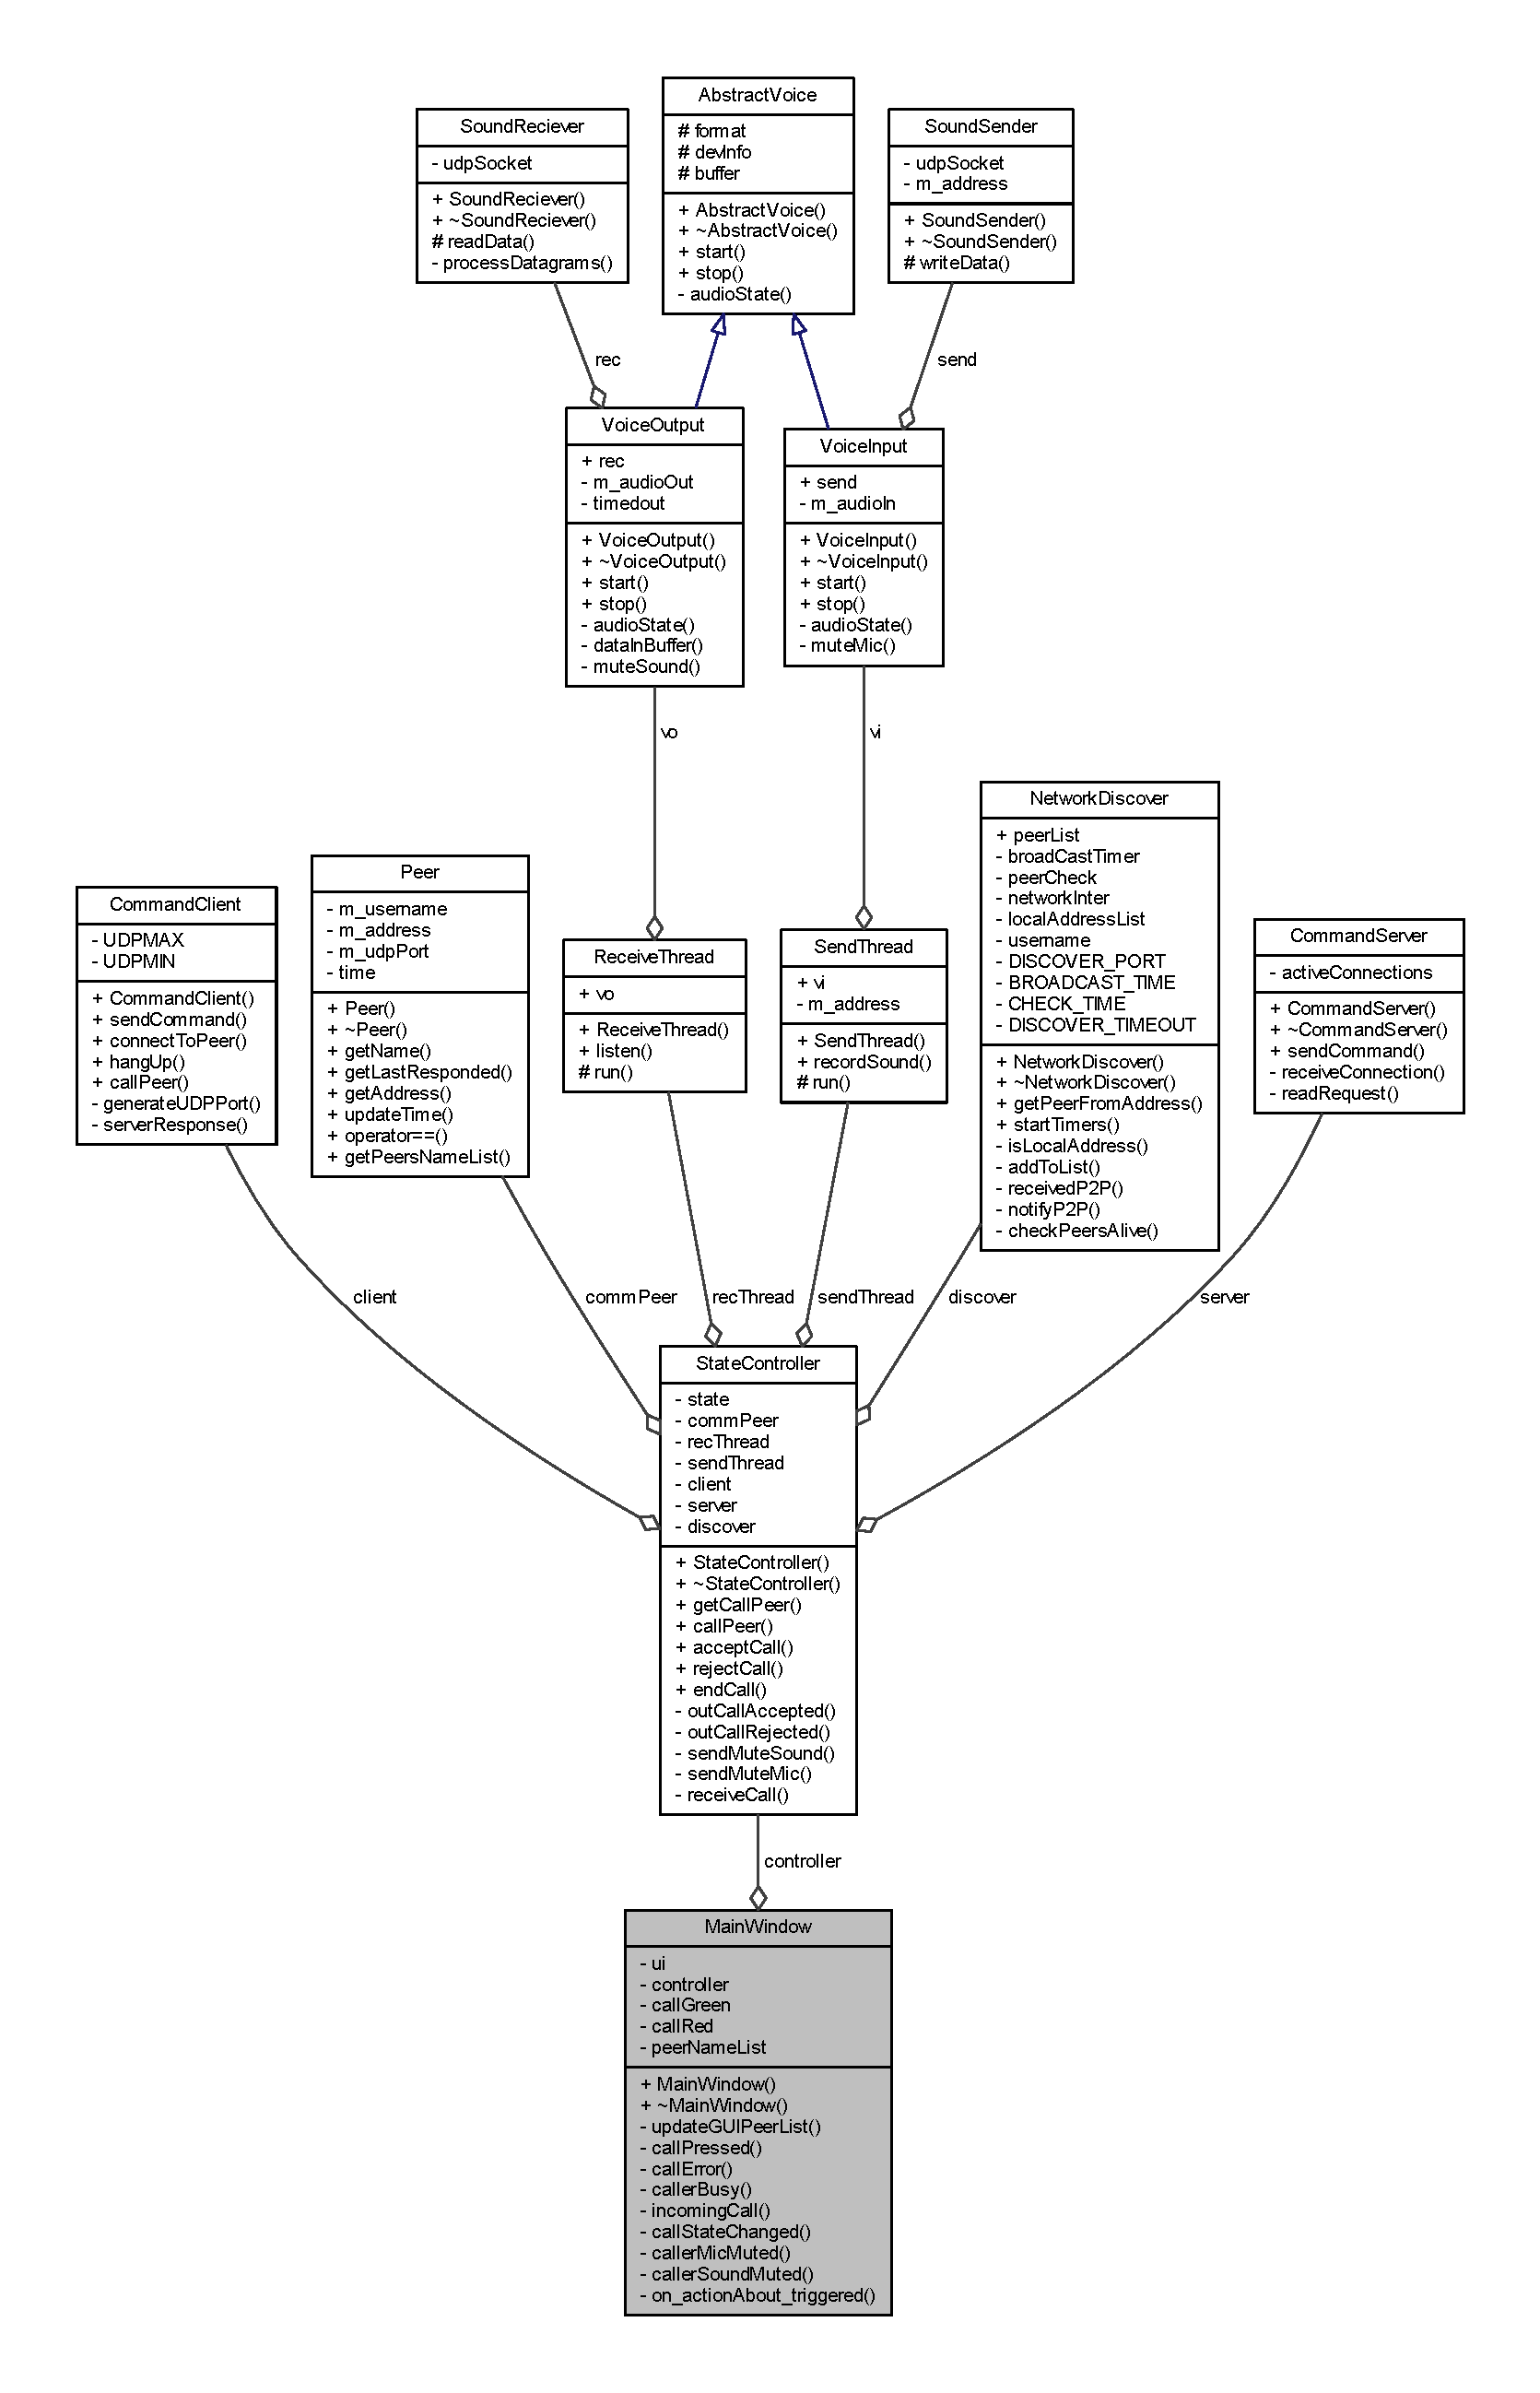
\includegraphics[width=350pt]{class_main_window__coll__graph}
\end{center}
\end{figure}
\subsection*{\-Signals}
\begin{DoxyCompactItemize}
\item 
void \hyperlink{class_main_window_aea2d395eaa1a1b353b7838731595a3f7}{call} (\-Q\-String)
\begin{DoxyCompactList}\small\item\em \-Signal emiited when the user has selected to start a new call. \end{DoxyCompactList}\item 
void \hyperlink{class_main_window_ac1ad769a26f328f8184cd63833af4539}{in\-Call\-Accepted} ()
\begin{DoxyCompactList}\small\item\em \-Informs anyone interested that the call was accepted. \end{DoxyCompactList}\item 
void \hyperlink{class_main_window_a3322ffd0516e30afc70f8b623301c426}{in\-Call\-Rejected} ()
\begin{DoxyCompactList}\small\item\em \-Informs anyone interested that the call was rejected. \end{DoxyCompactList}\end{DoxyCompactItemize}
\subsection*{\-Public \-Member \-Functions}
\begin{DoxyCompactItemize}
\item 
\hyperlink{class_main_window_a8b244be8b7b7db1b08de2a2acb9409db}{\-Main\-Window} (\-Q\-Widget $\ast$parent=0)
\begin{DoxyCompactList}\small\item\em \-Construction which sets up the \-U\-I class as well as all signals/slots and instansiates the controller. \end{DoxyCompactList}\item 
\hyperlink{class_main_window_ae98d00a93bc118200eeef9f9bba1dba7}{$\sim$\-Main\-Window} ()
\begin{DoxyCompactList}\small\item\em \-Default constructor which deletes the ui and all allocated objects. \end{DoxyCompactList}\end{DoxyCompactItemize}
\subsection*{\-Private \-Slots}
\begin{DoxyCompactItemize}
\item 
void \hyperlink{class_main_window_a780eb14bc5469aa2431a1d605a1bd431}{update\-G\-U\-I\-Peer\-List} (\-Q\-List$<$ \hyperlink{class_peer}{\-Peer} $\ast$ $>$ p\-List)
\begin{DoxyCompactList}\small\item\em \-Updates the graphical view of the peer list. \end{DoxyCompactList}\item 
void \hyperlink{class_main_window_afaa4ef4d091e0f4cf16036d831f30787}{call\-Pressed} ()
\begin{DoxyCompactList}\small\item\em \-User initiated a call. \end{DoxyCompactList}\item 
void \hyperlink{class_main_window_aed9515073081aa1f6cdb4949b5b11194}{call\-Error} (const \-Q\-String \&error)
\begin{DoxyCompactList}\small\item\em \-An error has occured for the user to be informed about. \end{DoxyCompactList}\item 
void \hyperlink{class_main_window_a342dc22be100ae360deb0fca0a0d610a}{caller\-Busy} ()
\begin{DoxyCompactList}\small\item\em \-The caller was busy, pop up dialog. \end{DoxyCompactList}\item 
void \hyperlink{class_main_window_a47e0e25f0b714888d25f3945b9f07185}{incoming\-Call} (const \-Q\-String \&caller)
\begin{DoxyCompactList}\small\item\em \-A new call is incoming, ask user's permission. \end{DoxyCompactList}\item 
void \hyperlink{class_main_window_ac473def8f3f23d0aa997355598be150b}{call\-State\-Changed} (\hyperlink{class_state_controller_a1aabd2155d8e6feb201ed3941e4ee2be}{\-State\-Controller\-::\-Vo\-I\-P\-State} state)
\begin{DoxyCompactList}\small\item\em \-Updates the \-G\-U\-I to reflect the new state. \end{DoxyCompactList}\item 
void \hyperlink{class_main_window_a4f308b9aade3aafea3c33773c17522aa}{caller\-Mic\-Muted} (bool)
\begin{DoxyCompactList}\small\item\em \-The caller has toggled their microphone. \end{DoxyCompactList}\item 
void \hyperlink{class_main_window_a73c0b86679333c83552253d798754e48}{caller\-Sound\-Muted} (bool)
\begin{DoxyCompactList}\small\item\em \-The caller has toggled their sound. \end{DoxyCompactList}\item 
void \hyperlink{class_main_window_a4f3ebda1ba39e0ef4d678b44893c9c7f}{on\-\_\-action\-About\-\_\-triggered} ()
\begin{DoxyCompactList}\small\item\em \-U\-I element to display information about the application. \end{DoxyCompactList}\end{DoxyCompactItemize}
\subsection*{\-Private \-Attributes}
\begin{DoxyCompactItemize}
\item 
\-Ui\-::\-Main\-Window $\ast$ \hyperlink{class_main_window_a35466a70ed47252a0191168126a352a5}{ui}
\begin{DoxyCompactList}\small\item\em \-U\-I class. \end{DoxyCompactList}\item 
\hyperlink{class_state_controller}{\-State\-Controller} $\ast$ \hyperlink{class_main_window_a998fca79d54f491c4ef158e03e8894d4}{controller}
\begin{DoxyCompactList}\small\item\em \-Controller resposible for all interaction. \end{DoxyCompactList}\item 
\-Q\-Pixmap \hyperlink{class_main_window_af6e038a052aefecc54322a166ad08bcf}{call\-Green}
\begin{DoxyCompactList}\small\item\em \-Green icon, showing in call. \end{DoxyCompactList}\item 
\-Q\-Pixmap \hyperlink{class_main_window_a9bd145f81a0a715e4739c3d893fb7b7b}{call\-Red}
\begin{DoxyCompactList}\small\item\em \-Red icon, showing out of call. \end{DoxyCompactList}\item 
\-Q\-String\-List \hyperlink{class_main_window_a8c245df1016600d0f111fb98c8738d6d}{peer\-Name\-List}
\begin{DoxyCompactList}\small\item\em \-A \-List of peers names to be displayed in a widget. \end{DoxyCompactList}\end{DoxyCompactItemize}


\subsection{\-Detailed \-Description}
\-Graphical interface class of type \-Q\-Main\-Window. 

\-This class instansiates and holds logic for the ui. \-It communicates with the state controller but has been made as decoupled as possible. 

\subsection{\-Constructor \& \-Destructor \-Documentation}
\hypertarget{class_main_window_a8b244be8b7b7db1b08de2a2acb9409db}{
\index{\-Main\-Window@{\-Main\-Window}!\-Main\-Window@{\-Main\-Window}}
\index{\-Main\-Window@{\-Main\-Window}!MainWindow@{\-Main\-Window}}
\subsubsection[{\-Main\-Window}]{\setlength{\rightskip}{0pt plus 5cm}\-Main\-Window\-::\-Main\-Window (
\begin{DoxyParamCaption}
\item[{\-Q\-Widget $\ast$}]{parent = {\ttfamily 0}}
\end{DoxyParamCaption}
)\hspace{0.3cm}{\ttfamily  \mbox{[}explicit\mbox{]}}}}
\label{class_main_window_a8b244be8b7b7db1b08de2a2acb9409db}


\-Construction which sets up the \-U\-I class as well as all signals/slots and instansiates the controller. 


\begin{DoxyParams}{\-Parameters}
{\em parent} & \-Parent for this object. \\
\hline
\end{DoxyParams}
\hypertarget{class_main_window_ae98d00a93bc118200eeef9f9bba1dba7}{
\index{\-Main\-Window@{\-Main\-Window}!$\sim$\-Main\-Window@{$\sim$\-Main\-Window}}
\index{$\sim$\-Main\-Window@{$\sim$\-Main\-Window}!MainWindow@{\-Main\-Window}}
\subsubsection[{$\sim$\-Main\-Window}]{\setlength{\rightskip}{0pt plus 5cm}\-Main\-Window\-::$\sim$\-Main\-Window (
\begin{DoxyParamCaption}
{}
\end{DoxyParamCaption}
)}}
\label{class_main_window_ae98d00a93bc118200eeef9f9bba1dba7}


\-Default constructor which deletes the ui and all allocated objects. 



\subsection{\-Member \-Function \-Documentation}
\hypertarget{class_main_window_aea2d395eaa1a1b353b7838731595a3f7}{
\index{\-Main\-Window@{\-Main\-Window}!call@{call}}
\index{call@{call}!MainWindow@{\-Main\-Window}}
\subsubsection[{call}]{\setlength{\rightskip}{0pt plus 5cm}void \-Main\-Window\-::call (
\begin{DoxyParamCaption}
\item[{\-Q\-String}]{}
\end{DoxyParamCaption}
)\hspace{0.3cm}{\ttfamily  \mbox{[}signal\mbox{]}}}}
\label{class_main_window_aea2d395eaa1a1b353b7838731595a3f7}


\-Signal emiited when the user has selected to start a new call. 

\-Provides the name selected. \hypertarget{class_main_window_a342dc22be100ae360deb0fca0a0d610a}{
\index{\-Main\-Window@{\-Main\-Window}!caller\-Busy@{caller\-Busy}}
\index{caller\-Busy@{caller\-Busy}!MainWindow@{\-Main\-Window}}
\subsubsection[{caller\-Busy}]{\setlength{\rightskip}{0pt plus 5cm}void \-Main\-Window\-::caller\-Busy (
\begin{DoxyParamCaption}
{}
\end{DoxyParamCaption}
)\hspace{0.3cm}{\ttfamily  \mbox{[}private, slot\mbox{]}}}}
\label{class_main_window_a342dc22be100ae360deb0fca0a0d610a}


\-The caller was busy, pop up dialog. 

\hypertarget{class_main_window_a4f308b9aade3aafea3c33773c17522aa}{
\index{\-Main\-Window@{\-Main\-Window}!caller\-Mic\-Muted@{caller\-Mic\-Muted}}
\index{caller\-Mic\-Muted@{caller\-Mic\-Muted}!MainWindow@{\-Main\-Window}}
\subsubsection[{caller\-Mic\-Muted}]{\setlength{\rightskip}{0pt plus 5cm}void \-Main\-Window\-::caller\-Mic\-Muted (
\begin{DoxyParamCaption}
\item[{bool}]{toggle}
\end{DoxyParamCaption}
)\hspace{0.3cm}{\ttfamily  \mbox{[}private, slot\mbox{]}}}}
\label{class_main_window_a4f308b9aade3aafea3c33773c17522aa}


\-The caller has toggled their microphone. 

\-This slot will updated the \-G\-U\-I accordingly. \hypertarget{class_main_window_aed9515073081aa1f6cdb4949b5b11194}{
\index{\-Main\-Window@{\-Main\-Window}!call\-Error@{call\-Error}}
\index{call\-Error@{call\-Error}!MainWindow@{\-Main\-Window}}
\subsubsection[{call\-Error}]{\setlength{\rightskip}{0pt plus 5cm}void \-Main\-Window\-::call\-Error (
\begin{DoxyParamCaption}
\item[{const \-Q\-String \&}]{error}
\end{DoxyParamCaption}
)\hspace{0.3cm}{\ttfamily  \mbox{[}private, slot\mbox{]}}}}
\label{class_main_window_aed9515073081aa1f6cdb4949b5b11194}


\-An error has occured for the user to be informed about. 

\-This will be popped up in a dialog. 
\begin{DoxyParams}{\-Parameters}
{\em error} & \-The error message. \\
\hline
\end{DoxyParams}
\hypertarget{class_main_window_a73c0b86679333c83552253d798754e48}{
\index{\-Main\-Window@{\-Main\-Window}!caller\-Sound\-Muted@{caller\-Sound\-Muted}}
\index{caller\-Sound\-Muted@{caller\-Sound\-Muted}!MainWindow@{\-Main\-Window}}
\subsubsection[{caller\-Sound\-Muted}]{\setlength{\rightskip}{0pt plus 5cm}void \-Main\-Window\-::caller\-Sound\-Muted (
\begin{DoxyParamCaption}
\item[{bool}]{toggle}
\end{DoxyParamCaption}
)\hspace{0.3cm}{\ttfamily  \mbox{[}private, slot\mbox{]}}}}
\label{class_main_window_a73c0b86679333c83552253d798754e48}


\-The caller has toggled their sound. 

\-This slot will updated the \-G\-U\-I accordingly. \hypertarget{class_main_window_afaa4ef4d091e0f4cf16036d831f30787}{
\index{\-Main\-Window@{\-Main\-Window}!call\-Pressed@{call\-Pressed}}
\index{call\-Pressed@{call\-Pressed}!MainWindow@{\-Main\-Window}}
\subsubsection[{call\-Pressed}]{\setlength{\rightskip}{0pt plus 5cm}void \-Main\-Window\-::call\-Pressed (
\begin{DoxyParamCaption}
{}
\end{DoxyParamCaption}
)\hspace{0.3cm}{\ttfamily  \mbox{[}private, slot\mbox{]}}}}
\label{class_main_window_afaa4ef4d091e0f4cf16036d831f30787}


\-User initiated a call. 

\hypertarget{class_main_window_ac473def8f3f23d0aa997355598be150b}{
\index{\-Main\-Window@{\-Main\-Window}!call\-State\-Changed@{call\-State\-Changed}}
\index{call\-State\-Changed@{call\-State\-Changed}!MainWindow@{\-Main\-Window}}
\subsubsection[{call\-State\-Changed}]{\setlength{\rightskip}{0pt plus 5cm}void \-Main\-Window\-::call\-State\-Changed (
\begin{DoxyParamCaption}
\item[{{\bf \-State\-Controller\-::\-Vo\-I\-P\-State}}]{state}
\end{DoxyParamCaption}
)\hspace{0.3cm}{\ttfamily  \mbox{[}private, slot\mbox{]}}}}
\label{class_main_window_ac473def8f3f23d0aa997355598be150b}


\-Updates the \-G\-U\-I to reflect the new state. 


\begin{DoxyParams}{\-Parameters}
{\em state} & \-The new state. \\
\hline
\end{DoxyParams}
\hypertarget{class_main_window_ac1ad769a26f328f8184cd63833af4539}{
\index{\-Main\-Window@{\-Main\-Window}!in\-Call\-Accepted@{in\-Call\-Accepted}}
\index{in\-Call\-Accepted@{in\-Call\-Accepted}!MainWindow@{\-Main\-Window}}
\subsubsection[{in\-Call\-Accepted}]{\setlength{\rightskip}{0pt plus 5cm}void \-Main\-Window\-::in\-Call\-Accepted (
\begin{DoxyParamCaption}
{}
\end{DoxyParamCaption}
)\hspace{0.3cm}{\ttfamily  \mbox{[}signal\mbox{]}}}}
\label{class_main_window_ac1ad769a26f328f8184cd63833af4539}


\-Informs anyone interested that the call was accepted. 

\hypertarget{class_main_window_a3322ffd0516e30afc70f8b623301c426}{
\index{\-Main\-Window@{\-Main\-Window}!in\-Call\-Rejected@{in\-Call\-Rejected}}
\index{in\-Call\-Rejected@{in\-Call\-Rejected}!MainWindow@{\-Main\-Window}}
\subsubsection[{in\-Call\-Rejected}]{\setlength{\rightskip}{0pt plus 5cm}void \-Main\-Window\-::in\-Call\-Rejected (
\begin{DoxyParamCaption}
{}
\end{DoxyParamCaption}
)\hspace{0.3cm}{\ttfamily  \mbox{[}signal\mbox{]}}}}
\label{class_main_window_a3322ffd0516e30afc70f8b623301c426}


\-Informs anyone interested that the call was rejected. 

\hypertarget{class_main_window_a47e0e25f0b714888d25f3945b9f07185}{
\index{\-Main\-Window@{\-Main\-Window}!incoming\-Call@{incoming\-Call}}
\index{incoming\-Call@{incoming\-Call}!MainWindow@{\-Main\-Window}}
\subsubsection[{incoming\-Call}]{\setlength{\rightskip}{0pt plus 5cm}void \-Main\-Window\-::incoming\-Call (
\begin{DoxyParamCaption}
\item[{const \-Q\-String \&}]{caller}
\end{DoxyParamCaption}
)\hspace{0.3cm}{\ttfamily  \mbox{[}private, slot\mbox{]}}}}
\label{class_main_window_a47e0e25f0b714888d25f3945b9f07185}


\-A new call is incoming, ask user's permission. 


\begin{DoxyParams}{\-Parameters}
{\em caller} & \-The name of the caller. \\
\hline
\end{DoxyParams}
\hypertarget{class_main_window_a4f3ebda1ba39e0ef4d678b44893c9c7f}{
\index{\-Main\-Window@{\-Main\-Window}!on\-\_\-action\-About\-\_\-triggered@{on\-\_\-action\-About\-\_\-triggered}}
\index{on\-\_\-action\-About\-\_\-triggered@{on\-\_\-action\-About\-\_\-triggered}!MainWindow@{\-Main\-Window}}
\subsubsection[{on\-\_\-action\-About\-\_\-triggered}]{\setlength{\rightskip}{0pt plus 5cm}void \-Main\-Window\-::on\-\_\-action\-About\-\_\-triggered (
\begin{DoxyParamCaption}
{}
\end{DoxyParamCaption}
)\hspace{0.3cm}{\ttfamily  \mbox{[}private, slot\mbox{]}}}}
\label{class_main_window_a4f3ebda1ba39e0ef4d678b44893c9c7f}


\-U\-I element to display information about the application. 

\hypertarget{class_main_window_a780eb14bc5469aa2431a1d605a1bd431}{
\index{\-Main\-Window@{\-Main\-Window}!update\-G\-U\-I\-Peer\-List@{update\-G\-U\-I\-Peer\-List}}
\index{update\-G\-U\-I\-Peer\-List@{update\-G\-U\-I\-Peer\-List}!MainWindow@{\-Main\-Window}}
\subsubsection[{update\-G\-U\-I\-Peer\-List}]{\setlength{\rightskip}{0pt plus 5cm}void \-Main\-Window\-::update\-G\-U\-I\-Peer\-List (
\begin{DoxyParamCaption}
\item[{\-Q\-List$<$ {\bf \-Peer} $\ast$ $>$}]{p\-List}
\end{DoxyParamCaption}
)\hspace{0.3cm}{\ttfamily  \mbox{[}private, slot\mbox{]}}}}
\label{class_main_window_a780eb14bc5469aa2431a1d605a1bd431}


\-Updates the graphical view of the peer list. 


\begin{DoxyParams}{\-Parameters}
{\em p\-List} & \-The list of peers. \\
\hline
\end{DoxyParams}


\subsection{\-Member \-Data \-Documentation}
\hypertarget{class_main_window_af6e038a052aefecc54322a166ad08bcf}{
\index{\-Main\-Window@{\-Main\-Window}!call\-Green@{call\-Green}}
\index{call\-Green@{call\-Green}!MainWindow@{\-Main\-Window}}
\subsubsection[{call\-Green}]{\setlength{\rightskip}{0pt plus 5cm}\-Q\-Pixmap {\bf \-Main\-Window\-::call\-Green}\hspace{0.3cm}{\ttfamily  \mbox{[}private\mbox{]}}}}
\label{class_main_window_af6e038a052aefecc54322a166ad08bcf}


\-Green icon, showing in call. 

\hypertarget{class_main_window_a9bd145f81a0a715e4739c3d893fb7b7b}{
\index{\-Main\-Window@{\-Main\-Window}!call\-Red@{call\-Red}}
\index{call\-Red@{call\-Red}!MainWindow@{\-Main\-Window}}
\subsubsection[{call\-Red}]{\setlength{\rightskip}{0pt plus 5cm}\-Q\-Pixmap {\bf \-Main\-Window\-::call\-Red}\hspace{0.3cm}{\ttfamily  \mbox{[}private\mbox{]}}}}
\label{class_main_window_a9bd145f81a0a715e4739c3d893fb7b7b}


\-Red icon, showing out of call. 

\hypertarget{class_main_window_a998fca79d54f491c4ef158e03e8894d4}{
\index{\-Main\-Window@{\-Main\-Window}!controller@{controller}}
\index{controller@{controller}!MainWindow@{\-Main\-Window}}
\subsubsection[{controller}]{\setlength{\rightskip}{0pt plus 5cm}{\bf \-State\-Controller}$\ast$ {\bf \-Main\-Window\-::controller}\hspace{0.3cm}{\ttfamily  \mbox{[}private\mbox{]}}}}
\label{class_main_window_a998fca79d54f491c4ef158e03e8894d4}


\-Controller resposible for all interaction. 

\hypertarget{class_main_window_a8c245df1016600d0f111fb98c8738d6d}{
\index{\-Main\-Window@{\-Main\-Window}!peer\-Name\-List@{peer\-Name\-List}}
\index{peer\-Name\-List@{peer\-Name\-List}!MainWindow@{\-Main\-Window}}
\subsubsection[{peer\-Name\-List}]{\setlength{\rightskip}{0pt plus 5cm}\-Q\-String\-List {\bf \-Main\-Window\-::peer\-Name\-List}\hspace{0.3cm}{\ttfamily  \mbox{[}private\mbox{]}}}}
\label{class_main_window_a8c245df1016600d0f111fb98c8738d6d}


\-A \-List of peers names to be displayed in a widget. 

\hypertarget{class_main_window_a35466a70ed47252a0191168126a352a5}{
\index{\-Main\-Window@{\-Main\-Window}!ui@{ui}}
\index{ui@{ui}!MainWindow@{\-Main\-Window}}
\subsubsection[{ui}]{\setlength{\rightskip}{0pt plus 5cm}\-Ui\-::\-Main\-Window$\ast$ {\bf \-Main\-Window\-::ui}\hspace{0.3cm}{\ttfamily  \mbox{[}private\mbox{]}}}}
\label{class_main_window_a35466a70ed47252a0191168126a352a5}


\-U\-I class. 



\-The documentation for this class was generated from the following files\-:\begin{DoxyCompactItemize}
\item 
\hyperlink{mainwindow_8h}{mainwindow.\-h}\item 
\hyperlink{mainwindow_8cpp}{mainwindow.\-cpp}\end{DoxyCompactItemize}

\hypertarget{class_network_discover}{
\section{\-Network\-Discover \-Class \-Reference}
\label{class_network_discover}\index{\-Network\-Discover@{\-Network\-Discover}}
}


\-Discovers local peers on the network to communicate with.  




{\ttfamily \#include $<$networkdiscover.\-h$>$}

\subsection*{\-Signals}
\begin{DoxyCompactItemize}
\item 
void \hyperlink{class_network_discover_a42566247e43198ea9cce91eb5f15511d}{peers\-Changed} (\-Q\-List$<$ \hyperlink{class_peer}{\-Peer} $\ast$ $>$)
\begin{DoxyCompactList}\small\item\em \-Emitted when the peer list has changed, ie. \end{DoxyCompactList}\end{DoxyCompactItemize}
\subsection*{\-Public \-Member \-Functions}
\begin{DoxyCompactItemize}
\item 
\hyperlink{class_network_discover_a35d97308463f9cbe622767b2d364bdbb}{\-Network\-Discover} (\-Q\-Object $\ast$parent=0)
\begin{DoxyCompactList}\small\item\em \-Gets local name, binds udp port, connects signals and slots and then starts timers. \end{DoxyCompactList}\item 
\hyperlink{class_network_discover_a416e23eb1f6925197596731e3c5f325e}{$\sim$\-Network\-Discover} ()
\begin{DoxyCompactList}\small\item\em \-Default destructor. \end{DoxyCompactList}\item 
\hyperlink{class_peer}{\-Peer} $\ast$ \hyperlink{class_network_discover_a91ec8539ddfeb90f6735d05f2f10b97a}{get\-Peer\-From\-Address} (const \-Q\-Host\-Address \&address)
\begin{DoxyCompactList}\small\item\em \-Returns a peer for an address. \end{DoxyCompactList}\item 
bool \hyperlink{class_network_discover_ac25855eb9d181d51c725a57f693d58f8}{start\-Timers} ()
\begin{DoxyCompactList}\small\item\em \-Starts the peer discovery timers. \end{DoxyCompactList}\end{DoxyCompactItemize}
\subsection*{\-Public \-Attributes}
\begin{DoxyCompactItemize}
\item 
\-Q\-Map$<$ \-Q\-String, \hyperlink{class_peer}{\-Peer} $\ast$ $>$ \hyperlink{class_network_discover_ac7f0c8a7a8e780c83c24b4fa8cbbbfef}{peer\-List}
\begin{DoxyCompactList}\small\item\em \-The list of peers currently detected on the network. \end{DoxyCompactList}\end{DoxyCompactItemize}
\subsection*{\-Private \-Slots}
\begin{DoxyCompactItemize}
\item 
void \hyperlink{class_network_discover_ada902f88ce4d9b1e707dfbf1be3e102c}{received\-P2\-P} ()
\begin{DoxyCompactList}\small\item\em \-Received peer signal from \-U\-D\-P port. \end{DoxyCompactList}\item 
void \hyperlink{class_network_discover_ac9c9e8988abe75fb02386b7783cf53be}{notify\-P2\-P} ()
\begin{DoxyCompactList}\small\item\em \-Broadcasts an identifier beacon via \-U\-D\-P. \end{DoxyCompactList}\item 
void \hyperlink{class_network_discover_aec820bf7bae99a2a8f533bb31a841ca6}{check\-Peers\-Alive} ()
\begin{DoxyCompactList}\small\item\em \-Periodically checks the last time a peer replied to our signal. \end{DoxyCompactList}\end{DoxyCompactItemize}
\subsection*{\-Private \-Member \-Functions}
\begin{DoxyCompactItemize}
\item 
bool \hyperlink{class_network_discover_ab1909b31fd4df24ebe095d3bbde3925e}{is\-Local\-Address} (\-Q\-Host\-Address)
\begin{DoxyCompactList}\small\item\em \-Detects if the address is local. \end{DoxyCompactList}\item 
bool \hyperlink{class_network_discover_a8e567964d959ba269d2570769eb7b1da}{add\-To\-List} (\-Q\-String $\ast$, \-Q\-Host\-Address $\ast$, quint16)
\begin{DoxyCompactList}\small\item\em \-Adds a peer to the list, with their name, address and their prefered communication port. \end{DoxyCompactList}\end{DoxyCompactItemize}
\subsection*{\-Private \-Attributes}
\begin{DoxyCompactItemize}
\item 
\-Q\-Timer \hyperlink{class_network_discover_a82d0981a5c6c1acecd85a0e210b631f2}{broad\-Cast\-Timer}
\begin{DoxyCompactList}\small\item\em \-Timer used to periodically broadcast that we are an alive peer. \end{DoxyCompactList}\item 
\-Q\-Timer \hyperlink{class_network_discover_ad23e0a7d95e0fed29acae8f193dfcfc3}{peer\-Check}
\begin{DoxyCompactList}\small\item\em \-Timer used to periodically check that our peers are still active. \end{DoxyCompactList}\item 
\-Q\-Network\-Interface \hyperlink{class_network_discover_a67c037cca501b587cc8c24ab5d971553}{network\-Inter}
\begin{DoxyCompactList}\small\item\em \-Used to obtain local network information. \end{DoxyCompactList}\item 
\-Q\-List$<$ \-Q\-Host\-Address $>$ \hyperlink{class_network_discover_a9db1fe648d568707cfcda8f00d2b5f5a}{local\-Address\-List}
\begin{DoxyCompactList}\small\item\em \-Local address list. \end{DoxyCompactList}\item 
\-Q\-String \hyperlink{class_network_discover_ad9dcef0352b63920211c0b442741bebb}{username}
\begin{DoxyCompactList}\small\item\em \-Local username detected. \end{DoxyCompactList}\end{DoxyCompactItemize}
\subsection*{\-Static \-Private \-Attributes}
\begin{DoxyCompactItemize}
\item 
static const int \hyperlink{class_network_discover_aae5acabb49790c03dd076c235fd3014c}{\-D\-I\-S\-C\-O\-V\-E\-R\-\_\-\-P\-O\-R\-T} = 45453
\begin{DoxyCompactList}\small\item\em \-The \-U\-D\-P port to be used for discovery. \end{DoxyCompactList}\item 
static const int \hyperlink{class_network_discover_ac85620fa17d1128dc86745611df1dbe0}{\-B\-R\-O\-A\-D\-C\-A\-S\-T\-\_\-\-T\-I\-M\-E} = 2000
\begin{DoxyCompactList}\small\item\em \-The time between broadcasting our signal in ms. \end{DoxyCompactList}\item 
static const int \hyperlink{class_network_discover_afc4903f686b81fff1247fc7cbcea17ff}{\-C\-H\-E\-C\-K\-\_\-\-T\-I\-M\-E} = 10000
\begin{DoxyCompactList}\small\item\em \-The time between checking our peers are still \char`\"{}alive\char`\"{}. \end{DoxyCompactList}\item 
static const int \hyperlink{class_network_discover_aebe784b2c4a47256321246c7d4fca5e6}{\-D\-I\-S\-C\-O\-V\-E\-R\-\_\-\-T\-I\-M\-E\-O\-U\-T} = 3000
\begin{DoxyCompactList}\small\item\em \-The time within that a peer should have last communicated. \end{DoxyCompactList}\end{DoxyCompactItemize}


\subsection{\-Detailed \-Description}
\-Discovers local peers on the network to communicate with. 

\-This class broadcasts and receives a beacon signal that is used to determine who is avaiable on the network for calling. \-A signal is sent out periodically to show an \char`\"{}alive\char`\"{} state. \-The same port is binded to listen to other peers, they are added to a list. \-Periodically a check is done to see the last know time of an update. \-This is used to remove peers from the list. \-This class inherits from \-Q\-Udp\-Socket. \begin{DoxySeeAlso}{\-See also}
\-Q\-Udp\-Socket 
\end{DoxySeeAlso}


\subsection{\-Constructor \& \-Destructor \-Documentation}
\hypertarget{class_network_discover_a35d97308463f9cbe622767b2d364bdbb}{
\index{\-Network\-Discover@{\-Network\-Discover}!\-Network\-Discover@{\-Network\-Discover}}
\index{\-Network\-Discover@{\-Network\-Discover}!NetworkDiscover@{\-Network\-Discover}}
\subsubsection[{\-Network\-Discover}]{\setlength{\rightskip}{0pt plus 5cm}\-Network\-Discover\-::\-Network\-Discover (
\begin{DoxyParamCaption}
\item[{\-Q\-Object $\ast$}]{parent = {\ttfamily 0}}
\end{DoxyParamCaption}
)\hspace{0.3cm}{\ttfamily  \mbox{[}explicit\mbox{]}}}}
\label{class_network_discover_a35d97308463f9cbe622767b2d364bdbb}


\-Gets local name, binds udp port, connects signals and slots and then starts timers. 


\begin{DoxyParams}{\-Parameters}
{\em parent} & \-Parent object. \\
\hline
\end{DoxyParams}
\hypertarget{class_network_discover_a416e23eb1f6925197596731e3c5f325e}{
\index{\-Network\-Discover@{\-Network\-Discover}!$\sim$\-Network\-Discover@{$\sim$\-Network\-Discover}}
\index{$\sim$\-Network\-Discover@{$\sim$\-Network\-Discover}!NetworkDiscover@{\-Network\-Discover}}
\subsubsection[{$\sim$\-Network\-Discover}]{\setlength{\rightskip}{0pt plus 5cm}\-Network\-Discover\-::$\sim$\-Network\-Discover (
\begin{DoxyParamCaption}
{}
\end{DoxyParamCaption}
)}}
\label{class_network_discover_a416e23eb1f6925197596731e3c5f325e}


\-Default destructor. 



\subsection{\-Member \-Function \-Documentation}
\hypertarget{class_network_discover_a8e567964d959ba269d2570769eb7b1da}{
\index{\-Network\-Discover@{\-Network\-Discover}!add\-To\-List@{add\-To\-List}}
\index{add\-To\-List@{add\-To\-List}!NetworkDiscover@{\-Network\-Discover}}
\subsubsection[{add\-To\-List}]{\setlength{\rightskip}{0pt plus 5cm}bool \-Network\-Discover\-::add\-To\-List (
\begin{DoxyParamCaption}
\item[{\-Q\-String $\ast$}]{sender\-Name, }
\item[{\-Q\-Host\-Address $\ast$}]{sender\-Address, }
\item[{quint16}]{port}
\end{DoxyParamCaption}
)\hspace{0.3cm}{\ttfamily  \mbox{[}private\mbox{]}}}}
\label{class_network_discover_a8e567964d959ba269d2570769eb7b1da}


\-Adds a peer to the list, with their name, address and their prefered communication port. 

\-Preferred port is not yet supported. \hypertarget{class_network_discover_aec820bf7bae99a2a8f533bb31a841ca6}{
\index{\-Network\-Discover@{\-Network\-Discover}!check\-Peers\-Alive@{check\-Peers\-Alive}}
\index{check\-Peers\-Alive@{check\-Peers\-Alive}!NetworkDiscover@{\-Network\-Discover}}
\subsubsection[{check\-Peers\-Alive}]{\setlength{\rightskip}{0pt plus 5cm}void \-Network\-Discover\-::check\-Peers\-Alive (
\begin{DoxyParamCaption}
{}
\end{DoxyParamCaption}
)\hspace{0.3cm}{\ttfamily  \mbox{[}private, slot\mbox{]}}}}
\label{class_network_discover_aec820bf7bae99a2a8f533bb31a841ca6}


\-Periodically checks the last time a peer replied to our signal. 

\-If it is more than a threshold, they are removed. \hypertarget{class_network_discover_a91ec8539ddfeb90f6735d05f2f10b97a}{
\index{\-Network\-Discover@{\-Network\-Discover}!get\-Peer\-From\-Address@{get\-Peer\-From\-Address}}
\index{get\-Peer\-From\-Address@{get\-Peer\-From\-Address}!NetworkDiscover@{\-Network\-Discover}}
\subsubsection[{get\-Peer\-From\-Address}]{\setlength{\rightskip}{0pt plus 5cm}{\bf \-Peer} $\ast$ \-Network\-Discover\-::get\-Peer\-From\-Address (
\begin{DoxyParamCaption}
\item[{const \-Q\-Host\-Address \&}]{address}
\end{DoxyParamCaption}
)}}
\label{class_network_discover_a91ec8539ddfeb90f6735d05f2f10b97a}


\-Returns a peer for an address. 


\begin{DoxyParams}{\-Parameters}
{\em address} & \-The address for the peer. \\
\hline
\end{DoxyParams}
\begin{DoxyReturn}{\-Returns}
\-The returned peer or null. 
\end{DoxyReturn}
\hypertarget{class_network_discover_ab1909b31fd4df24ebe095d3bbde3925e}{
\index{\-Network\-Discover@{\-Network\-Discover}!is\-Local\-Address@{is\-Local\-Address}}
\index{is\-Local\-Address@{is\-Local\-Address}!NetworkDiscover@{\-Network\-Discover}}
\subsubsection[{is\-Local\-Address}]{\setlength{\rightskip}{0pt plus 5cm}bool \-Network\-Discover\-::is\-Local\-Address (
\begin{DoxyParamCaption}
\item[{\-Q\-Host\-Address}]{sender\-Address}
\end{DoxyParamCaption}
)\hspace{0.3cm}{\ttfamily  \mbox{[}private\mbox{]}}}}
\label{class_network_discover_ab1909b31fd4df24ebe095d3bbde3925e}


\-Detects if the address is local. 

\-This method can be called to see if the broadcast message is actually us, we do this by checking all our local addresses against the one received. \hypertarget{class_network_discover_ac9c9e8988abe75fb02386b7783cf53be}{
\index{\-Network\-Discover@{\-Network\-Discover}!notify\-P2\-P@{notify\-P2\-P}}
\index{notify\-P2\-P@{notify\-P2\-P}!NetworkDiscover@{\-Network\-Discover}}
\subsubsection[{notify\-P2\-P}]{\setlength{\rightskip}{0pt plus 5cm}void \-Network\-Discover\-::notify\-P2\-P (
\begin{DoxyParamCaption}
{}
\end{DoxyParamCaption}
)\hspace{0.3cm}{\ttfamily  \mbox{[}private, slot\mbox{]}}}}
\label{class_network_discover_ac9c9e8988abe75fb02386b7783cf53be}


\-Broadcasts an identifier beacon via \-U\-D\-P. 

\-The broadcast is done periodically on a timer. \hypertarget{class_network_discover_a42566247e43198ea9cce91eb5f15511d}{
\index{\-Network\-Discover@{\-Network\-Discover}!peers\-Changed@{peers\-Changed}}
\index{peers\-Changed@{peers\-Changed}!NetworkDiscover@{\-Network\-Discover}}
\subsubsection[{peers\-Changed}]{\setlength{\rightskip}{0pt plus 5cm}void \-Network\-Discover\-::peers\-Changed (
\begin{DoxyParamCaption}
\item[{\-Q\-List$<$ {\bf \-Peer} $\ast$ $>$}]{}
\end{DoxyParamCaption}
)\hspace{0.3cm}{\ttfamily  \mbox{[}signal\mbox{]}}}}
\label{class_network_discover_a42566247e43198ea9cce91eb5f15511d}


\-Emitted when the peer list has changed, ie. 

new peer or removed peer. \hypertarget{class_network_discover_ada902f88ce4d9b1e707dfbf1be3e102c}{
\index{\-Network\-Discover@{\-Network\-Discover}!received\-P2\-P@{received\-P2\-P}}
\index{received\-P2\-P@{received\-P2\-P}!NetworkDiscover@{\-Network\-Discover}}
\subsubsection[{received\-P2\-P}]{\setlength{\rightskip}{0pt plus 5cm}void \-Network\-Discover\-::received\-P2\-P (
\begin{DoxyParamCaption}
{}
\end{DoxyParamCaption}
)\hspace{0.3cm}{\ttfamily  \mbox{[}private, slot\mbox{]}}}}
\label{class_network_discover_ada902f88ce4d9b1e707dfbf1be3e102c}


\-Received peer signal from \-U\-D\-P port. 

\-Check its id against our maintained list. is\-Local\-Address(sender\-Address)) \{ \hypertarget{class_network_discover_ac25855eb9d181d51c725a57f693d58f8}{
\index{\-Network\-Discover@{\-Network\-Discover}!start\-Timers@{start\-Timers}}
\index{start\-Timers@{start\-Timers}!NetworkDiscover@{\-Network\-Discover}}
\subsubsection[{start\-Timers}]{\setlength{\rightskip}{0pt plus 5cm}bool \-Network\-Discover\-::start\-Timers (
\begin{DoxyParamCaption}
{}
\end{DoxyParamCaption}
)}}
\label{class_network_discover_ac25855eb9d181d51c725a57f693d58f8}


\-Starts the peer discovery timers. 

\-Starts the peer alive check timer and the broadcast timer. \begin{DoxyReturn}{\-Returns}
\-Returns if timers were started successfully. 
\end{DoxyReturn}


\subsection{\-Member \-Data \-Documentation}
\hypertarget{class_network_discover_ac85620fa17d1128dc86745611df1dbe0}{
\index{\-Network\-Discover@{\-Network\-Discover}!\-B\-R\-O\-A\-D\-C\-A\-S\-T\-\_\-\-T\-I\-M\-E@{\-B\-R\-O\-A\-D\-C\-A\-S\-T\-\_\-\-T\-I\-M\-E}}
\index{\-B\-R\-O\-A\-D\-C\-A\-S\-T\-\_\-\-T\-I\-M\-E@{\-B\-R\-O\-A\-D\-C\-A\-S\-T\-\_\-\-T\-I\-M\-E}!NetworkDiscover@{\-Network\-Discover}}
\subsubsection[{\-B\-R\-O\-A\-D\-C\-A\-S\-T\-\_\-\-T\-I\-M\-E}]{\setlength{\rightskip}{0pt plus 5cm}const int {\bf \-Network\-Discover\-::\-B\-R\-O\-A\-D\-C\-A\-S\-T\-\_\-\-T\-I\-M\-E} = 2000\hspace{0.3cm}{\ttfamily  \mbox{[}static, private\mbox{]}}}}
\label{class_network_discover_ac85620fa17d1128dc86745611df1dbe0}


\-The time between broadcasting our signal in ms. 

\hypertarget{class_network_discover_a82d0981a5c6c1acecd85a0e210b631f2}{
\index{\-Network\-Discover@{\-Network\-Discover}!broad\-Cast\-Timer@{broad\-Cast\-Timer}}
\index{broad\-Cast\-Timer@{broad\-Cast\-Timer}!NetworkDiscover@{\-Network\-Discover}}
\subsubsection[{broad\-Cast\-Timer}]{\setlength{\rightskip}{0pt plus 5cm}\-Q\-Timer {\bf \-Network\-Discover\-::broad\-Cast\-Timer}\hspace{0.3cm}{\ttfamily  \mbox{[}private\mbox{]}}}}
\label{class_network_discover_a82d0981a5c6c1acecd85a0e210b631f2}


\-Timer used to periodically broadcast that we are an alive peer. 

\hypertarget{class_network_discover_afc4903f686b81fff1247fc7cbcea17ff}{
\index{\-Network\-Discover@{\-Network\-Discover}!\-C\-H\-E\-C\-K\-\_\-\-T\-I\-M\-E@{\-C\-H\-E\-C\-K\-\_\-\-T\-I\-M\-E}}
\index{\-C\-H\-E\-C\-K\-\_\-\-T\-I\-M\-E@{\-C\-H\-E\-C\-K\-\_\-\-T\-I\-M\-E}!NetworkDiscover@{\-Network\-Discover}}
\subsubsection[{\-C\-H\-E\-C\-K\-\_\-\-T\-I\-M\-E}]{\setlength{\rightskip}{0pt plus 5cm}const int {\bf \-Network\-Discover\-::\-C\-H\-E\-C\-K\-\_\-\-T\-I\-M\-E} = 10000\hspace{0.3cm}{\ttfamily  \mbox{[}static, private\mbox{]}}}}
\label{class_network_discover_afc4903f686b81fff1247fc7cbcea17ff}


\-The time between checking our peers are still \char`\"{}alive\char`\"{}. 

\hypertarget{class_network_discover_aae5acabb49790c03dd076c235fd3014c}{
\index{\-Network\-Discover@{\-Network\-Discover}!\-D\-I\-S\-C\-O\-V\-E\-R\-\_\-\-P\-O\-R\-T@{\-D\-I\-S\-C\-O\-V\-E\-R\-\_\-\-P\-O\-R\-T}}
\index{\-D\-I\-S\-C\-O\-V\-E\-R\-\_\-\-P\-O\-R\-T@{\-D\-I\-S\-C\-O\-V\-E\-R\-\_\-\-P\-O\-R\-T}!NetworkDiscover@{\-Network\-Discover}}
\subsubsection[{\-D\-I\-S\-C\-O\-V\-E\-R\-\_\-\-P\-O\-R\-T}]{\setlength{\rightskip}{0pt plus 5cm}const int {\bf \-Network\-Discover\-::\-D\-I\-S\-C\-O\-V\-E\-R\-\_\-\-P\-O\-R\-T} = 45453\hspace{0.3cm}{\ttfamily  \mbox{[}static, private\mbox{]}}}}
\label{class_network_discover_aae5acabb49790c03dd076c235fd3014c}


\-The \-U\-D\-P port to be used for discovery. 

\hypertarget{class_network_discover_aebe784b2c4a47256321246c7d4fca5e6}{
\index{\-Network\-Discover@{\-Network\-Discover}!\-D\-I\-S\-C\-O\-V\-E\-R\-\_\-\-T\-I\-M\-E\-O\-U\-T@{\-D\-I\-S\-C\-O\-V\-E\-R\-\_\-\-T\-I\-M\-E\-O\-U\-T}}
\index{\-D\-I\-S\-C\-O\-V\-E\-R\-\_\-\-T\-I\-M\-E\-O\-U\-T@{\-D\-I\-S\-C\-O\-V\-E\-R\-\_\-\-T\-I\-M\-E\-O\-U\-T}!NetworkDiscover@{\-Network\-Discover}}
\subsubsection[{\-D\-I\-S\-C\-O\-V\-E\-R\-\_\-\-T\-I\-M\-E\-O\-U\-T}]{\setlength{\rightskip}{0pt plus 5cm}const int {\bf \-Network\-Discover\-::\-D\-I\-S\-C\-O\-V\-E\-R\-\_\-\-T\-I\-M\-E\-O\-U\-T} = 3000\hspace{0.3cm}{\ttfamily  \mbox{[}static, private\mbox{]}}}}
\label{class_network_discover_aebe784b2c4a47256321246c7d4fca5e6}


\-The time within that a peer should have last communicated. 

\hypertarget{class_network_discover_a9db1fe648d568707cfcda8f00d2b5f5a}{
\index{\-Network\-Discover@{\-Network\-Discover}!local\-Address\-List@{local\-Address\-List}}
\index{local\-Address\-List@{local\-Address\-List}!NetworkDiscover@{\-Network\-Discover}}
\subsubsection[{local\-Address\-List}]{\setlength{\rightskip}{0pt plus 5cm}\-Q\-List$<$\-Q\-Host\-Address$>$ {\bf \-Network\-Discover\-::local\-Address\-List}\hspace{0.3cm}{\ttfamily  \mbox{[}private\mbox{]}}}}
\label{class_network_discover_a9db1fe648d568707cfcda8f00d2b5f5a}


\-Local address list. 

\hypertarget{class_network_discover_a67c037cca501b587cc8c24ab5d971553}{
\index{\-Network\-Discover@{\-Network\-Discover}!network\-Inter@{network\-Inter}}
\index{network\-Inter@{network\-Inter}!NetworkDiscover@{\-Network\-Discover}}
\subsubsection[{network\-Inter}]{\setlength{\rightskip}{0pt plus 5cm}\-Q\-Network\-Interface {\bf \-Network\-Discover\-::network\-Inter}\hspace{0.3cm}{\ttfamily  \mbox{[}private\mbox{]}}}}
\label{class_network_discover_a67c037cca501b587cc8c24ab5d971553}


\-Used to obtain local network information. 

\hypertarget{class_network_discover_ad23e0a7d95e0fed29acae8f193dfcfc3}{
\index{\-Network\-Discover@{\-Network\-Discover}!peer\-Check@{peer\-Check}}
\index{peer\-Check@{peer\-Check}!NetworkDiscover@{\-Network\-Discover}}
\subsubsection[{peer\-Check}]{\setlength{\rightskip}{0pt plus 5cm}\-Q\-Timer {\bf \-Network\-Discover\-::peer\-Check}\hspace{0.3cm}{\ttfamily  \mbox{[}private\mbox{]}}}}
\label{class_network_discover_ad23e0a7d95e0fed29acae8f193dfcfc3}


\-Timer used to periodically check that our peers are still active. 

\hypertarget{class_network_discover_ac7f0c8a7a8e780c83c24b4fa8cbbbfef}{
\index{\-Network\-Discover@{\-Network\-Discover}!peer\-List@{peer\-List}}
\index{peer\-List@{peer\-List}!NetworkDiscover@{\-Network\-Discover}}
\subsubsection[{peer\-List}]{\setlength{\rightskip}{0pt plus 5cm}\-Q\-Map$<$\-Q\-String,{\bf \-Peer}$\ast$$>$ {\bf \-Network\-Discover\-::peer\-List}}}
\label{class_network_discover_ac7f0c8a7a8e780c83c24b4fa8cbbbfef}


\-The list of peers currently detected on the network. 

\hypertarget{class_network_discover_ad9dcef0352b63920211c0b442741bebb}{
\index{\-Network\-Discover@{\-Network\-Discover}!username@{username}}
\index{username@{username}!NetworkDiscover@{\-Network\-Discover}}
\subsubsection[{username}]{\setlength{\rightskip}{0pt plus 5cm}\-Q\-String {\bf \-Network\-Discover\-::username}\hspace{0.3cm}{\ttfamily  \mbox{[}private\mbox{]}}}}
\label{class_network_discover_ad9dcef0352b63920211c0b442741bebb}


\-Local username detected. 



\-The documentation for this class was generated from the following files\-:\begin{DoxyCompactItemize}
\item 
\hyperlink{networkdiscover_8h}{networkdiscover.\-h}\item 
\hyperlink{networkdiscover_8cpp}{networkdiscover.\-cpp}\end{DoxyCompactItemize}

\hypertarget{class_peer}{
\section{\-Peer \-Class \-Reference}
\label{class_peer}\index{\-Peer@{\-Peer}}
}


\-Holds information for a located communication peer on the network.  




{\ttfamily \#include $<$peer.\-h$>$}

\subsection*{\-Public \-Member \-Functions}
\begin{DoxyCompactItemize}
\item 
\hyperlink{class_peer_a3360b580084c61a8bc31144ae2af912a}{\-Peer} (\-Q\-Object $\ast$parent, \-Q\-String $\ast$name, \-Q\-Host\-Address $\ast$address, quint16 port)
\begin{DoxyCompactList}\small\item\em \-Constructs a new peer. \end{DoxyCompactList}\item 
\-Q\-String \hyperlink{class_peer_ad66666aca923fe13b4cca3f836d12fa7}{get\-Name} () const 
\begin{DoxyCompactList}\small\item\em \-Returns the username of peer. \end{DoxyCompactList}\item 
\-Q\-Time \hyperlink{class_peer_a1c9797749ddfbb9261e93f51cc3ace9e}{get\-Last\-Responded} ()
\begin{DoxyCompactList}\small\item\em \-Gets the time the peer last communicated with us. \end{DoxyCompactList}\item 
\-Q\-Host\-Address $\ast$ \hyperlink{class_peer_ac1e626629eeaaeebff30f2eda36c3a5e}{get\-Address} ()
\begin{DoxyCompactList}\small\item\em \-Returns the \-I\-P address of the peer. \end{DoxyCompactList}\item 
\hypertarget{class_peer_a49f70d43a1822edaeb8f3f7de66b12e3}{
void \hyperlink{class_peer_a49f70d43a1822edaeb8f3f7de66b12e3}{update\-Time} ()}
\label{class_peer_a49f70d43a1822edaeb8f3f7de66b12e3}

\begin{DoxyCompactList}\small\item\em \-Updates the peers last communication time with the current local system time. \end{DoxyCompactList}\item 
\hypertarget{class_peer_afa304e14507579b7f3aaf8b2e7483f1a}{
bool \hyperlink{class_peer_afa304e14507579b7f3aaf8b2e7483f1a}{operator==} (const \hyperlink{class_peer}{\-Peer} \&peer)}
\label{class_peer_afa304e14507579b7f3aaf8b2e7483f1a}

\begin{DoxyCompactList}\small\item\em \-Compares two peers by their username. \end{DoxyCompactList}\end{DoxyCompactItemize}
\subsection*{\-Static \-Public \-Member \-Functions}
\begin{DoxyCompactItemize}
\item 
static \-Q\-String\-List \hyperlink{class_peer_ab728eb8f441b3473983d9dfd902d8ac9}{get\-Peers\-Name\-List} (const \-Q\-List$<$ \hyperlink{class_peer}{\-Peer} $\ast$ $>$ \&peer\-List)
\begin{DoxyCompactList}\small\item\em \-Static method that obtains a list of usernames from a list of peers. \end{DoxyCompactList}\end{DoxyCompactItemize}


\subsection{\-Detailed \-Description}
\-Holds information for a located communication peer on the network. 

\-A \hyperlink{class_peer}{\-Peer} is someone on the same network who is also broad casting to discover other users of this application. \-This class represents their username and address. 

\subsection{\-Constructor \& \-Destructor \-Documentation}
\hypertarget{class_peer_a3360b580084c61a8bc31144ae2af912a}{
\index{\-Peer@{\-Peer}!\-Peer@{\-Peer}}
\index{\-Peer@{\-Peer}!Peer@{\-Peer}}
\subsubsection[{\-Peer}]{\setlength{\rightskip}{0pt plus 5cm}\-Peer\-::\-Peer (
\begin{DoxyParamCaption}
\item[{\-Q\-Object $\ast$}]{parent, }
\item[{\-Q\-String $\ast$}]{name, }
\item[{\-Q\-Host\-Address $\ast$}]{address, }
\item[{quint16}]{port}
\end{DoxyParamCaption}
)\hspace{0.3cm}{\ttfamily  \mbox{[}explicit\mbox{]}}}}
\label{class_peer_a3360b580084c61a8bc31144ae2af912a}


\-Constructs a new peer. 


\begin{DoxyParams}{\-Parameters}
{\em parent} & \-Parent object. \\
\hline
{\em name} & \-The username of the peer. \\
\hline
{\em address} & \-The \-I\-P of the peer. \\
\hline
{\em port} & \-The prefered voice chat udp port for the peer. \-This is \-N\-O\-T implemented yet. \\
\hline
\end{DoxyParams}


\subsection{\-Member \-Function \-Documentation}
\hypertarget{class_peer_ac1e626629eeaaeebff30f2eda36c3a5e}{
\index{\-Peer@{\-Peer}!get\-Address@{get\-Address}}
\index{get\-Address@{get\-Address}!Peer@{\-Peer}}
\subsubsection[{get\-Address}]{\setlength{\rightskip}{0pt plus 5cm}\-Q\-Host\-Address$\ast$ \-Peer\-::get\-Address (
\begin{DoxyParamCaption}
{}
\end{DoxyParamCaption}
)\hspace{0.3cm}{\ttfamily  \mbox{[}inline\mbox{]}}}}
\label{class_peer_ac1e626629eeaaeebff30f2eda36c3a5e}


\-Returns the \-I\-P address of the peer. 

\begin{DoxyReturn}{\-Returns}
\-The \-I\-P address. 
\end{DoxyReturn}
\hypertarget{class_peer_a1c9797749ddfbb9261e93f51cc3ace9e}{
\index{\-Peer@{\-Peer}!get\-Last\-Responded@{get\-Last\-Responded}}
\index{get\-Last\-Responded@{get\-Last\-Responded}!Peer@{\-Peer}}
\subsubsection[{get\-Last\-Responded}]{\setlength{\rightskip}{0pt plus 5cm}\-Q\-Time \-Peer\-::get\-Last\-Responded (
\begin{DoxyParamCaption}
{}
\end{DoxyParamCaption}
)\hspace{0.3cm}{\ttfamily  \mbox{[}inline\mbox{]}}}}
\label{class_peer_a1c9797749ddfbb9261e93f51cc3ace9e}


\-Gets the time the peer last communicated with us. 

\begin{DoxyReturn}{\-Returns}
\-The time of last communication. 
\end{DoxyReturn}
\hypertarget{class_peer_ad66666aca923fe13b4cca3f836d12fa7}{
\index{\-Peer@{\-Peer}!get\-Name@{get\-Name}}
\index{get\-Name@{get\-Name}!Peer@{\-Peer}}
\subsubsection[{get\-Name}]{\setlength{\rightskip}{0pt plus 5cm}\-Q\-String \-Peer\-::get\-Name (
\begin{DoxyParamCaption}
{}
\end{DoxyParamCaption}
) const\hspace{0.3cm}{\ttfamily  \mbox{[}inline\mbox{]}}}}
\label{class_peer_ad66666aca923fe13b4cca3f836d12fa7}


\-Returns the username of peer. 

\begin{DoxyReturn}{\-Returns}
\-The username of the peer. 
\end{DoxyReturn}
\hypertarget{class_peer_ab728eb8f441b3473983d9dfd902d8ac9}{
\index{\-Peer@{\-Peer}!get\-Peers\-Name\-List@{get\-Peers\-Name\-List}}
\index{get\-Peers\-Name\-List@{get\-Peers\-Name\-List}!Peer@{\-Peer}}
\subsubsection[{get\-Peers\-Name\-List}]{\setlength{\rightskip}{0pt plus 5cm}\-Q\-String\-List \-Peer\-::get\-Peers\-Name\-List (
\begin{DoxyParamCaption}
\item[{const \-Q\-List$<$ {\bf \-Peer} $\ast$ $>$ \&}]{peer\-List}
\end{DoxyParamCaption}
)\hspace{0.3cm}{\ttfamily  \mbox{[}static\mbox{]}}}}
\label{class_peer_ab728eb8f441b3473983d9dfd902d8ac9}


\-Static method that obtains a list of usernames from a list of peers. 


\begin{DoxyParams}{\-Parameters}
{\em peer\-List} & \-The list of peers. \\
\hline
\end{DoxyParams}
\begin{DoxyReturn}{\-Returns}
\-A \-Stringlist containing all usernames of peers. 
\end{DoxyReturn}


\-The documentation for this class was generated from the following files\-:\begin{DoxyCompactItemize}
\item 
peer.\-h\item 
peer.\-cpp\end{DoxyCompactItemize}

\hypertarget{class_receive_thread}{
\section{\-Receive\-Thread \-Class \-Reference}
\label{class_receive_thread}\index{\-Receive\-Thread@{\-Receive\-Thread}}
}


\-A \-Thread class that controls listening for incoming voice data.  




{\ttfamily \#include $<$receivethread.\-h$>$}



\-Collaboration diagram for \-Receive\-Thread\-:\nopagebreak
\begin{figure}[H]
\begin{center}
\leavevmode
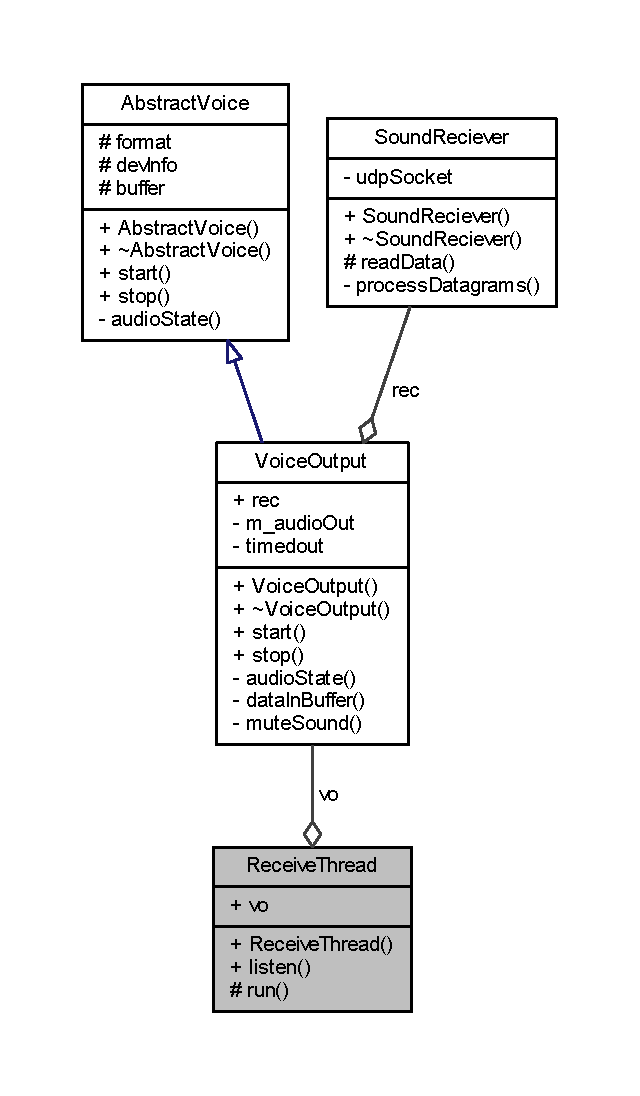
\includegraphics[width=307pt]{class_receive_thread__coll__graph}
\end{center}
\end{figure}
\subsection*{\-Public \-Slots}
\begin{DoxyCompactItemize}
\item 
void \hyperlink{class_receive_thread_a0eb5b7ab172cf0a35fee1e499d1a04e2}{listen} ()
\begin{DoxyCompactList}\small\item\em \-Starts the new thread. \end{DoxyCompactList}\end{DoxyCompactItemize}
\subsection*{\-Signals}
\begin{DoxyCompactItemize}
\item 
void \hyperlink{class_receive_thread_a971403a676eb058555b5099f04a5b546}{mute\-Sound} (bool)
\begin{DoxyCompactList}\small\item\em \-Signal that should emitted when a request to mute is processed. \end{DoxyCompactList}\end{DoxyCompactItemize}
\subsection*{\-Public \-Member \-Functions}
\begin{DoxyCompactItemize}
\item 
\hyperlink{class_receive_thread_a7d3037d96e9f4f93850026dca7ff0787}{\-Receive\-Thread} (\-Q\-Object $\ast$parent=0)
\begin{DoxyCompactList}\small\item\em \-Default constructor. \end{DoxyCompactList}\end{DoxyCompactItemize}
\subsection*{\-Public \-Attributes}
\begin{DoxyCompactItemize}
\item 
\hyperlink{class_voice_output}{\-Voice\-Output} \hyperlink{class_receive_thread_ab1d07e023e07536515ae30c8991822a7}{vo}
\end{DoxyCompactItemize}
\subsection*{\-Protected \-Member \-Functions}
\begin{DoxyCompactItemize}
\item 
void \hyperlink{class_receive_thread_a5033e892e97f8fe46d25c5da6bd15674}{run} ()
\begin{DoxyCompactList}\small\item\em \-Reimplmented function from \-Q\-Thread that beings receiving and playback. \end{DoxyCompactList}\end{DoxyCompactItemize}


\subsection{\-Detailed \-Description}
\-A \-Thread class that controls listening for incoming voice data. 

\-This class listens for incoming \-U\-D\-P and then plays it using the \-Computers default audio out device. \-This class inherits from \-Q\-Thread. 

\subsection{\-Constructor \& \-Destructor \-Documentation}
\hypertarget{class_receive_thread_a7d3037d96e9f4f93850026dca7ff0787}{
\index{\-Receive\-Thread@{\-Receive\-Thread}!\-Receive\-Thread@{\-Receive\-Thread}}
\index{\-Receive\-Thread@{\-Receive\-Thread}!ReceiveThread@{\-Receive\-Thread}}
\subsubsection[{\-Receive\-Thread}]{\setlength{\rightskip}{0pt plus 5cm}\-Receive\-Thread\-::\-Receive\-Thread (
\begin{DoxyParamCaption}
\item[{\-Q\-Object $\ast$}]{parent = {\ttfamily 0}}
\end{DoxyParamCaption}
)\hspace{0.3cm}{\ttfamily  \mbox{[}explicit\mbox{]}}}}
\label{class_receive_thread_a7d3037d96e9f4f93850026dca7ff0787}


\-Default constructor. 


\begin{DoxyParams}{\-Parameters}
{\em parent} & \-The owner of this object. \\
\hline
\end{DoxyParams}


\subsection{\-Member \-Function \-Documentation}
\hypertarget{class_receive_thread_a0eb5b7ab172cf0a35fee1e499d1a04e2}{
\index{\-Receive\-Thread@{\-Receive\-Thread}!listen@{listen}}
\index{listen@{listen}!ReceiveThread@{\-Receive\-Thread}}
\subsubsection[{listen}]{\setlength{\rightskip}{0pt plus 5cm}void \-Receive\-Thread\-::listen (
\begin{DoxyParamCaption}
{}
\end{DoxyParamCaption}
)\hspace{0.3cm}{\ttfamily  \mbox{[}slot\mbox{]}}}}
\label{class_receive_thread_a0eb5b7ab172cf0a35fee1e499d1a04e2}


\-Starts the new thread. 

\hypertarget{class_receive_thread_a971403a676eb058555b5099f04a5b546}{
\index{\-Receive\-Thread@{\-Receive\-Thread}!mute\-Sound@{mute\-Sound}}
\index{mute\-Sound@{mute\-Sound}!ReceiveThread@{\-Receive\-Thread}}
\subsubsection[{mute\-Sound}]{\setlength{\rightskip}{0pt plus 5cm}void \-Receive\-Thread\-::mute\-Sound (
\begin{DoxyParamCaption}
\item[{bool}]{}
\end{DoxyParamCaption}
)\hspace{0.3cm}{\ttfamily  \mbox{[}signal\mbox{]}}}}
\label{class_receive_thread_a971403a676eb058555b5099f04a5b546}


\-Signal that should emitted when a request to mute is processed. 

\-This class will then mute the sound. \hypertarget{class_receive_thread_a5033e892e97f8fe46d25c5da6bd15674}{
\index{\-Receive\-Thread@{\-Receive\-Thread}!run@{run}}
\index{run@{run}!ReceiveThread@{\-Receive\-Thread}}
\subsubsection[{run}]{\setlength{\rightskip}{0pt plus 5cm}void \-Receive\-Thread\-::run (
\begin{DoxyParamCaption}
{}
\end{DoxyParamCaption}
)\hspace{0.3cm}{\ttfamily  \mbox{[}protected\mbox{]}}}}
\label{class_receive_thread_a5033e892e97f8fe46d25c5da6bd15674}


\-Reimplmented function from \-Q\-Thread that beings receiving and playback. 



\subsection{\-Member \-Data \-Documentation}
\hypertarget{class_receive_thread_ab1d07e023e07536515ae30c8991822a7}{
\index{\-Receive\-Thread@{\-Receive\-Thread}!vo@{vo}}
\index{vo@{vo}!ReceiveThread@{\-Receive\-Thread}}
\subsubsection[{vo}]{\setlength{\rightskip}{0pt plus 5cm}{\bf \-Voice\-Output} {\bf \-Receive\-Thread\-::vo}}}
\label{class_receive_thread_ab1d07e023e07536515ae30c8991822a7}


\-The documentation for this class was generated from the following files\-:\begin{DoxyCompactItemize}
\item 
\hyperlink{receivethread_8h}{receivethread.\-h}\item 
\hyperlink{receivethread_8cpp}{receivethread.\-cpp}\end{DoxyCompactItemize}

\hypertarget{class_send_thread}{
\section{\-Send\-Thread \-Class \-Reference}
\label{class_send_thread}\index{\-Send\-Thread@{\-Send\-Thread}}
}


\-A \-Thread class that controls recording audio and sending data communication.  




{\ttfamily \#include $<$sendthread.\-h$>$}



\-Collaboration diagram for \-Send\-Thread\-:\nopagebreak
\begin{figure}[H]
\begin{center}
\leavevmode
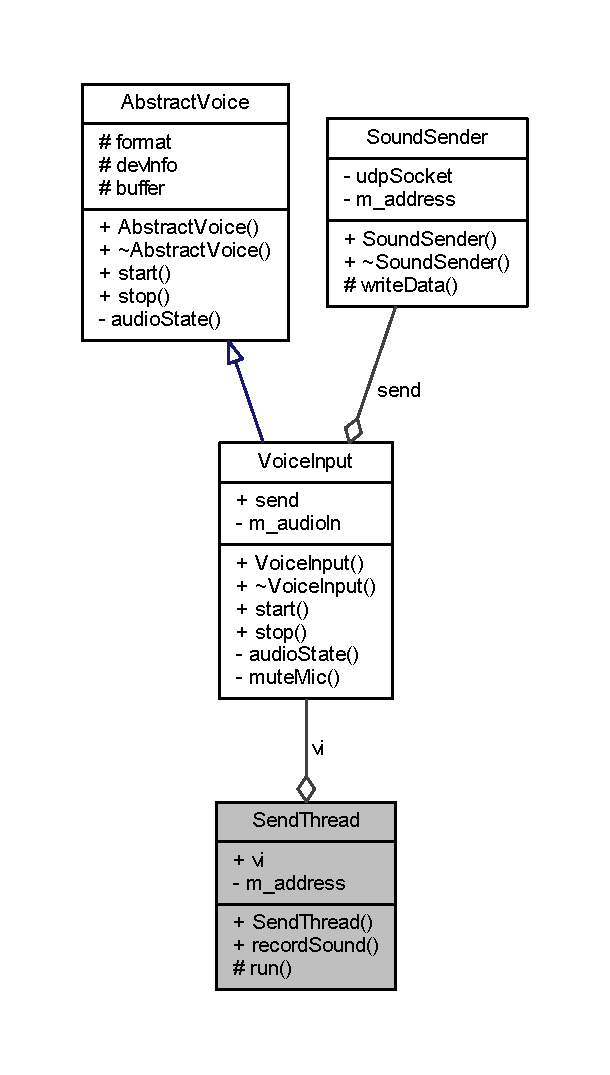
\includegraphics[width=293pt]{class_send_thread__coll__graph}
\end{center}
\end{figure}
\subsection*{\-Public \-Slots}
\begin{DoxyCompactItemize}
\item 
void \hyperlink{class_send_thread_ace7f54d057aea7d6ef58949333095f35}{record\-Sound} (const \-Q\-Host\-Address \&address)
\begin{DoxyCompactList}\small\item\em \-Starts the new thread, sending data to the given address. \end{DoxyCompactList}\end{DoxyCompactItemize}
\subsection*{\-Signals}
\begin{DoxyCompactItemize}
\item 
void \hyperlink{class_send_thread_afff2d01a9c3f193f68840d8bfc3af83d}{mute\-Mic} (bool)
\begin{DoxyCompactList}\small\item\em \-Signal that should emitted when a request to mute the mic is processed. \end{DoxyCompactList}\end{DoxyCompactItemize}
\subsection*{\-Public \-Member \-Functions}
\begin{DoxyCompactItemize}
\item 
\hyperlink{class_send_thread_a69eb38313a68a80b495277f05fa4f7ca}{\-Send\-Thread} (\-Q\-Object $\ast$parent=0)
\begin{DoxyCompactList}\small\item\em \-Default constructor. \end{DoxyCompactList}\end{DoxyCompactItemize}
\subsection*{\-Public \-Attributes}
\begin{DoxyCompactItemize}
\item 
\hyperlink{class_voice_input}{\-Voice\-Input} \hyperlink{class_send_thread_a8b1a2012e2ead9ab029c4e55b49b5d6b}{vi}
\end{DoxyCompactItemize}
\subsection*{\-Protected \-Member \-Functions}
\begin{DoxyCompactItemize}
\item 
void \hyperlink{class_send_thread_a7d389ce773db570613325fb56fb19e9a}{run} ()
\begin{DoxyCompactList}\small\item\em \-Reimplmented function from \-Q\-Thread that beings receiving and playback. \end{DoxyCompactList}\end{DoxyCompactItemize}
\subsection*{\-Private \-Attributes}
\begin{DoxyCompactItemize}
\item 
\-Q\-Host\-Address \hyperlink{class_send_thread_a7902661ef7e43bc4b0e17b0166530e87}{m\-\_\-address}
\begin{DoxyCompactList}\small\item\em locally stored address for thread access. \end{DoxyCompactList}\end{DoxyCompactItemize}


\subsection{\-Detailed \-Description}
\-A \-Thread class that controls recording audio and sending data communication. 

\-This class records audio from the default recording device and the sends them via \-U\-D\-P to the destination specified. \-This class inherits from \-Q\-Thread. 

\subsection{\-Constructor \& \-Destructor \-Documentation}
\hypertarget{class_send_thread_a69eb38313a68a80b495277f05fa4f7ca}{
\index{\-Send\-Thread@{\-Send\-Thread}!\-Send\-Thread@{\-Send\-Thread}}
\index{\-Send\-Thread@{\-Send\-Thread}!SendThread@{\-Send\-Thread}}
\subsubsection[{\-Send\-Thread}]{\setlength{\rightskip}{0pt plus 5cm}\-Send\-Thread\-::\-Send\-Thread (
\begin{DoxyParamCaption}
\item[{\-Q\-Object $\ast$}]{parent = {\ttfamily 0}}
\end{DoxyParamCaption}
)\hspace{0.3cm}{\ttfamily  \mbox{[}explicit\mbox{]}}}}
\label{class_send_thread_a69eb38313a68a80b495277f05fa4f7ca}


\-Default constructor. 


\begin{DoxyParams}{\-Parameters}
{\em parent} & \-The owner of this object. \\
\hline
\end{DoxyParams}


\subsection{\-Member \-Function \-Documentation}
\hypertarget{class_send_thread_afff2d01a9c3f193f68840d8bfc3af83d}{
\index{\-Send\-Thread@{\-Send\-Thread}!mute\-Mic@{mute\-Mic}}
\index{mute\-Mic@{mute\-Mic}!SendThread@{\-Send\-Thread}}
\subsubsection[{mute\-Mic}]{\setlength{\rightskip}{0pt plus 5cm}void \-Send\-Thread\-::mute\-Mic (
\begin{DoxyParamCaption}
\item[{bool}]{}
\end{DoxyParamCaption}
)\hspace{0.3cm}{\ttfamily  \mbox{[}signal\mbox{]}}}}
\label{class_send_thread_afff2d01a9c3f193f68840d8bfc3af83d}


\-Signal that should emitted when a request to mute the mic is processed. 

\-This class will then mute the microphone. \hypertarget{class_send_thread_ace7f54d057aea7d6ef58949333095f35}{
\index{\-Send\-Thread@{\-Send\-Thread}!record\-Sound@{record\-Sound}}
\index{record\-Sound@{record\-Sound}!SendThread@{\-Send\-Thread}}
\subsubsection[{record\-Sound}]{\setlength{\rightskip}{0pt plus 5cm}void \-Send\-Thread\-::record\-Sound (
\begin{DoxyParamCaption}
\item[{const \-Q\-Host\-Address \&}]{address}
\end{DoxyParamCaption}
)\hspace{0.3cm}{\ttfamily  \mbox{[}slot\mbox{]}}}}
\label{class_send_thread_ace7f54d057aea7d6ef58949333095f35}


\-Starts the new thread, sending data to the given address. 


\begin{DoxyParams}{\-Parameters}
{\em address} & \-The address to send the recorded audio. \\
\hline
\end{DoxyParams}
\hypertarget{class_send_thread_a7d389ce773db570613325fb56fb19e9a}{
\index{\-Send\-Thread@{\-Send\-Thread}!run@{run}}
\index{run@{run}!SendThread@{\-Send\-Thread}}
\subsubsection[{run}]{\setlength{\rightskip}{0pt plus 5cm}void \-Send\-Thread\-::run (
\begin{DoxyParamCaption}
{}
\end{DoxyParamCaption}
)\hspace{0.3cm}{\ttfamily  \mbox{[}protected\mbox{]}}}}
\label{class_send_thread_a7d389ce773db570613325fb56fb19e9a}


\-Reimplmented function from \-Q\-Thread that beings receiving and playback. 



\subsection{\-Member \-Data \-Documentation}
\hypertarget{class_send_thread_a7902661ef7e43bc4b0e17b0166530e87}{
\index{\-Send\-Thread@{\-Send\-Thread}!m\-\_\-address@{m\-\_\-address}}
\index{m\-\_\-address@{m\-\_\-address}!SendThread@{\-Send\-Thread}}
\subsubsection[{m\-\_\-address}]{\setlength{\rightskip}{0pt plus 5cm}\-Q\-Host\-Address {\bf \-Send\-Thread\-::m\-\_\-address}\hspace{0.3cm}{\ttfamily  \mbox{[}private\mbox{]}}}}
\label{class_send_thread_a7902661ef7e43bc4b0e17b0166530e87}


locally stored address for thread access. 

\hypertarget{class_send_thread_a8b1a2012e2ead9ab029c4e55b49b5d6b}{
\index{\-Send\-Thread@{\-Send\-Thread}!vi@{vi}}
\index{vi@{vi}!SendThread@{\-Send\-Thread}}
\subsubsection[{vi}]{\setlength{\rightskip}{0pt plus 5cm}{\bf \-Voice\-Input} {\bf \-Send\-Thread\-::vi}}}
\label{class_send_thread_a8b1a2012e2ead9ab029c4e55b49b5d6b}


\-The documentation for this class was generated from the following files\-:\begin{DoxyCompactItemize}
\item 
\hyperlink{sendthread_8h}{sendthread.\-h}\item 
\hyperlink{sendthread_8cpp}{sendthread.\-cpp}\end{DoxyCompactItemize}

\hypertarget{class_sound_reciever}{
\section{\-Sound\-Reciever \-Class \-Reference}
\label{class_sound_reciever}\index{\-Sound\-Reciever@{\-Sound\-Reciever}}
}


\-A buffer that receives \-U\-D\-P audio data over the network.  




{\ttfamily \#include $<$soundreciever.\-h$>$}

\subsection*{\-Public \-Member \-Functions}
\begin{DoxyCompactItemize}
\item 
\hyperlink{class_sound_reciever_ad10126bf26dd00c6a48d763c9691e0ca}{\-Sound\-Reciever} (\-Q\-Object $\ast$parent=0)
\begin{DoxyCompactList}\small\item\em \-Default constructor which binds to a \-U\-D\-P port. \end{DoxyCompactList}\item 
\hypertarget{class_sound_reciever_ae7e8a754e275fedf25e4cc8f86f64d72}{
\hyperlink{class_sound_reciever_ae7e8a754e275fedf25e4cc8f86f64d72}{$\sim$\-Sound\-Reciever} ()}
\label{class_sound_reciever_ae7e8a754e275fedf25e4cc8f86f64d72}

\begin{DoxyCompactList}\small\item\em \-Deletes the \-U\-D\-P\-Socket. \end{DoxyCompactList}\end{DoxyCompactItemize}
\subsection*{\-Protected \-Member \-Functions}
\begin{DoxyCompactItemize}
\item 
qint64 \hyperlink{class_sound_reciever_ad2e6e099486057cce325d4775c499eb9}{read\-Data} (char $\ast$data, qint64 len)
\begin{DoxyCompactList}\small\item\em \-Overridden \-Q\-Buffer method. \end{DoxyCompactList}\end{DoxyCompactItemize}


\subsection{\-Detailed \-Description}
\-A buffer that receives \-U\-D\-P audio data over the network. 

\-This class listens on a specific \-U\-D\-P port for audio data sent by another client. \-It decompresses it and adds it to it's buffer. \-Read requests on this buffer will empty it. \-This class inherits from \-Q\-Buffer. 

\subsection{\-Constructor \& \-Destructor \-Documentation}
\hypertarget{class_sound_reciever_ad10126bf26dd00c6a48d763c9691e0ca}{
\index{\-Sound\-Reciever@{\-Sound\-Reciever}!\-Sound\-Reciever@{\-Sound\-Reciever}}
\index{\-Sound\-Reciever@{\-Sound\-Reciever}!SoundReciever@{\-Sound\-Reciever}}
\subsubsection[{\-Sound\-Reciever}]{\setlength{\rightskip}{0pt plus 5cm}\-Sound\-Reciever\-::\-Sound\-Reciever (
\begin{DoxyParamCaption}
\item[{\-Q\-Object $\ast$}]{parent = {\ttfamily 0}}
\end{DoxyParamCaption}
)\hspace{0.3cm}{\ttfamily  \mbox{[}explicit\mbox{]}}}}
\label{class_sound_reciever_ad10126bf26dd00c6a48d763c9691e0ca}


\-Default constructor which binds to a \-U\-D\-P port. 


\begin{DoxyParams}{\-Parameters}
{\em parent} & \-The owner of this object. \\
\hline
\end{DoxyParams}


\subsection{\-Member \-Function \-Documentation}
\hypertarget{class_sound_reciever_ad2e6e099486057cce325d4775c499eb9}{
\index{\-Sound\-Reciever@{\-Sound\-Reciever}!read\-Data@{read\-Data}}
\index{read\-Data@{read\-Data}!SoundReciever@{\-Sound\-Reciever}}
\subsubsection[{read\-Data}]{\setlength{\rightskip}{0pt plus 5cm}qint64 \-Sound\-Reciever\-::read\-Data (
\begin{DoxyParamCaption}
\item[{char $\ast$}]{data, }
\item[{qint64}]{len}
\end{DoxyParamCaption}
)\hspace{0.3cm}{\ttfamily  \mbox{[}protected\mbox{]}}}}
\label{class_sound_reciever_ad2e6e099486057cce325d4775c499eb9}


\-Overridden \-Q\-Buffer method. 

\-This method will empty the buffer on a read request. 
\begin{DoxyParams}{\-Parameters}
{\em data} & \-A pointer to data where it should be placed. \\
\hline
{\em len} & \-The length of data to try and read \\
\hline
\end{DoxyParams}
\begin{DoxyReturn}{\-Returns}
\-The length actually read into data. 
\end{DoxyReturn}
\begin{DoxySeeAlso}{\-See also}
\-Q\-Buffer\-::read\-Data() 
\end{DoxySeeAlso}


\-The documentation for this class was generated from the following files\-:\begin{DoxyCompactItemize}
\item 
soundreciever.\-h\item 
soundreciever.\-cpp\end{DoxyCompactItemize}

\hypertarget{class_sound_sender}{
\section{\-Sound\-Sender \-Class \-Reference}
\label{class_sound_sender}\index{\-Sound\-Sender@{\-Sound\-Sender}}
}


\-A buffer that sends \-U\-D\-P audio data over the network.  




{\ttfamily \#include $<$soundsender.\-h$>$}

\subsection*{\-Public \-Member \-Functions}
\begin{DoxyCompactItemize}
\item 
\hyperlink{class_sound_sender_a15a16cf2d16d1de5de0f0d0e4b4ce5c9}{\-Sound\-Sender} (\-Q\-Object $\ast$parent, \-Q\-Host\-Address address)
\begin{DoxyCompactList}\small\item\em \-Default constructor which binds to a \-U\-D\-P port. \end{DoxyCompactList}\item 
\hyperlink{class_sound_sender_a15f4c11ed7d489972876697b776b27ab}{$\sim$\-Sound\-Sender} ()
\begin{DoxyCompactList}\small\item\em \-Deletes the \-U\-D\-P\-Socket. \end{DoxyCompactList}\end{DoxyCompactItemize}
\subsection*{\-Protected \-Member \-Functions}
\begin{DoxyCompactItemize}
\item 
qint64 \hyperlink{class_sound_sender_a2557d162440651dcee73996162d4820a}{write\-Data} (const char $\ast$data, qint64 len)
\begin{DoxyCompactList}\small\item\em \-Overridden from \-Q\-Buffer, when data is written to this buffer it is sent down the network to the address specified. \end{DoxyCompactList}\end{DoxyCompactItemize}
\subsection*{\-Private \-Attributes}
\begin{DoxyCompactItemize}
\item 
\-Q\-Udp\-Socket $\ast$ \hyperlink{class_sound_sender_a00386335e797a20af7a64a77871553ae}{udp\-Socket}
\begin{DoxyCompactList}\small\item\em \-The udp socket used. \end{DoxyCompactList}\item 
\-Q\-Host\-Address \hyperlink{class_sound_sender_aa2046b227bcc7cf1be86aabd197aaa3f}{m\-\_\-address}
\begin{DoxyCompactList}\small\item\em \-The address to send the data. \end{DoxyCompactList}\end{DoxyCompactItemize}


\subsection{\-Detailed \-Description}
\-A buffer that sends \-U\-D\-P audio data over the network. 

\-This class sends audio data down a specific \-U\-D\-P port to another client. \-When data is written to this buffer, it is immenditely compressed and sent down the network. 

\subsection{\-Constructor \& \-Destructor \-Documentation}
\hypertarget{class_sound_sender_a15a16cf2d16d1de5de0f0d0e4b4ce5c9}{
\index{\-Sound\-Sender@{\-Sound\-Sender}!\-Sound\-Sender@{\-Sound\-Sender}}
\index{\-Sound\-Sender@{\-Sound\-Sender}!SoundSender@{\-Sound\-Sender}}
\subsubsection[{\-Sound\-Sender}]{\setlength{\rightskip}{0pt plus 5cm}\-Sound\-Sender\-::\-Sound\-Sender (
\begin{DoxyParamCaption}
\item[{\-Q\-Object $\ast$}]{parent, }
\item[{\-Q\-Host\-Address}]{address}
\end{DoxyParamCaption}
)\hspace{0.3cm}{\ttfamily  \mbox{[}explicit\mbox{]}}}}
\label{class_sound_sender_a15a16cf2d16d1de5de0f0d0e4b4ce5c9}


\-Default constructor which binds to a \-U\-D\-P port. 


\begin{DoxyParams}{\-Parameters}
{\em parent} & \-The owner of this object. \\
\hline
{\em address} & \-The address to send the data. \\
\hline
\end{DoxyParams}
\hypertarget{class_sound_sender_a15f4c11ed7d489972876697b776b27ab}{
\index{\-Sound\-Sender@{\-Sound\-Sender}!$\sim$\-Sound\-Sender@{$\sim$\-Sound\-Sender}}
\index{$\sim$\-Sound\-Sender@{$\sim$\-Sound\-Sender}!SoundSender@{\-Sound\-Sender}}
\subsubsection[{$\sim$\-Sound\-Sender}]{\setlength{\rightskip}{0pt plus 5cm}\-Sound\-Sender\-::$\sim$\-Sound\-Sender (
\begin{DoxyParamCaption}
{}
\end{DoxyParamCaption}
)}}
\label{class_sound_sender_a15f4c11ed7d489972876697b776b27ab}


\-Deletes the \-U\-D\-P\-Socket. 



\subsection{\-Member \-Function \-Documentation}
\hypertarget{class_sound_sender_a2557d162440651dcee73996162d4820a}{
\index{\-Sound\-Sender@{\-Sound\-Sender}!write\-Data@{write\-Data}}
\index{write\-Data@{write\-Data}!SoundSender@{\-Sound\-Sender}}
\subsubsection[{write\-Data}]{\setlength{\rightskip}{0pt plus 5cm}qint64 \-Sound\-Sender\-::write\-Data (
\begin{DoxyParamCaption}
\item[{const char $\ast$}]{data, }
\item[{qint64}]{len}
\end{DoxyParamCaption}
)\hspace{0.3cm}{\ttfamily  \mbox{[}protected\mbox{]}}}}
\label{class_sound_sender_a2557d162440651dcee73996162d4820a}


\-Overridden from \-Q\-Buffer, when data is written to this buffer it is sent down the network to the address specified. 


\begin{DoxyParams}{\-Parameters}
{\em data} & \-The data to put into the buffer. \\
\hline
{\em len} & \-The length of data to add. \\
\hline
\end{DoxyParams}
\begin{DoxyReturn}{\-Returns}
\-The length of data sent. 
\end{DoxyReturn}


\subsection{\-Member \-Data \-Documentation}
\hypertarget{class_sound_sender_aa2046b227bcc7cf1be86aabd197aaa3f}{
\index{\-Sound\-Sender@{\-Sound\-Sender}!m\-\_\-address@{m\-\_\-address}}
\index{m\-\_\-address@{m\-\_\-address}!SoundSender@{\-Sound\-Sender}}
\subsubsection[{m\-\_\-address}]{\setlength{\rightskip}{0pt plus 5cm}\-Q\-Host\-Address {\bf \-Sound\-Sender\-::m\-\_\-address}\hspace{0.3cm}{\ttfamily  \mbox{[}private\mbox{]}}}}
\label{class_sound_sender_aa2046b227bcc7cf1be86aabd197aaa3f}


\-The address to send the data. 

\hypertarget{class_sound_sender_a00386335e797a20af7a64a77871553ae}{
\index{\-Sound\-Sender@{\-Sound\-Sender}!udp\-Socket@{udp\-Socket}}
\index{udp\-Socket@{udp\-Socket}!SoundSender@{\-Sound\-Sender}}
\subsubsection[{udp\-Socket}]{\setlength{\rightskip}{0pt plus 5cm}\-Q\-Udp\-Socket$\ast$ {\bf \-Sound\-Sender\-::udp\-Socket}\hspace{0.3cm}{\ttfamily  \mbox{[}private\mbox{]}}}}
\label{class_sound_sender_a00386335e797a20af7a64a77871553ae}


\-The udp socket used. 



\-The documentation for this class was generated from the following files\-:\begin{DoxyCompactItemize}
\item 
\hyperlink{soundsender_8h}{soundsender.\-h}\item 
\hyperlink{soundsender_8cpp}{soundsender.\-cpp}\end{DoxyCompactItemize}

\hypertarget{class_state_controller}{
\section{\-State\-Controller \-Class \-Reference}
\label{class_state_controller}\index{\-State\-Controller@{\-State\-Controller}}
}


\-This controller object contains state information and acts as a go between the view and model.  




{\ttfamily \#include $<$statecontroller.\-h$>$}

\subsection*{\-Public \-Types}
\begin{DoxyCompactItemize}
\item 
enum \hyperlink{class_state_controller_a1aabd2155d8e6feb201ed3941e4ee2be}{\-Vo\-I\-P\-State} \{ \hyperlink{class_state_controller_a1aabd2155d8e6feb201ed3941e4ee2beaaa2246adace3ba467ba59ca67820f4cc}{\-Ready}, 
\hyperlink{class_state_controller_a1aabd2155d8e6feb201ed3941e4ee2beae99363dcdf7f911223e5e75d348832d4}{\-Calling}, 
\hyperlink{class_state_controller_a1aabd2155d8e6feb201ed3941e4ee2beadee615ec66e7823e546668a00c857c13}{\-In\-Call}
 \}
\begin{DoxyCompactList}\small\item\em \-Possible \-Vo\-I\-P states for the application to be in. \end{DoxyCompactList}\end{DoxyCompactItemize}
\subsection*{\-Public \-Slots}
\begin{DoxyCompactItemize}
\item 
void \hyperlink{class_state_controller_ac2d1ccb2bab7565fee787a87580cdb83}{call\-Peer} (\-Q\-String name)
\begin{DoxyCompactList}\small\item\em \-U\-Is should connect to this slot with the name of the person they wish to call, the controller will initiate the call. \end{DoxyCompactList}\item 
void \hyperlink{class_state_controller_a7ae34b3ab2c5189c2e216ef78fae6a7e}{accept\-Call} ()
\begin{DoxyCompactList}\small\item\em \-U\-Is should conect to this slot when they wish to accept a call. \end{DoxyCompactList}\item 
void \hyperlink{class_state_controller_a0898c62cc514101cda35ee08618368b8}{reject\-Call} ()
\begin{DoxyCompactList}\small\item\em \-U\-Is should conect to this slot when they wish to reject a call. \end{DoxyCompactList}\item 
void \hyperlink{class_state_controller_aa82e7568aed9fc5d1e13f7ed94535abf}{end\-Call} ()
\begin{DoxyCompactList}\small\item\em \-U\-Is should conect to this slot when they wish to end a call. \end{DoxyCompactList}\end{DoxyCompactItemize}
\subsection*{\-Signals}
\begin{DoxyCompactItemize}
\item 
void \hyperlink{class_state_controller_a6db599925ca114fd1f1d0204a8de75ec}{update\-Peer\-List} (\-Q\-List$<$ \hyperlink{class_peer}{\-Peer} $\ast$ $>$)
\begin{DoxyCompactList}\small\item\em \-Signal emitted when an updated peer list is available . \end{DoxyCompactList}\item 
void \hyperlink{class_state_controller_aaf4d11ecaef3d8872a9c93b5b3e5af3b}{call\-Incoming} (\-Q\-String)
\begin{DoxyCompactList}\small\item\em \-Signal emitted when a call is being requested to initiate. \end{DoxyCompactList}\item 
void \hyperlink{class_state_controller_a393dbc547e29ffad28daa44517481ca5}{caller\-Busy} ()
\begin{DoxyCompactList}\small\item\em \-Emitted when a call was initiated but the caller was busy. \end{DoxyCompactList}\item 
void \hyperlink{class_state_controller_acff9d9f23348247c6844f4b198b6ba23}{new\-State} (\hyperlink{class_state_controller_a1aabd2155d8e6feb201ed3941e4ee2be}{\-State\-Controller\-::\-Vo\-I\-P\-State})
\begin{DoxyCompactList}\small\item\em \-The application has entered a new state. \end{DoxyCompactList}\item 
void \hyperlink{class_state_controller_ab7c03a4203338d1f17e95758ad96647c}{mute\-Sound} (bool)
\begin{DoxyCompactList}\small\item\em \-User has initiated that their sound has been toggled, this signal will be emitted and a message sent to caller. \end{DoxyCompactList}\item 
void \hyperlink{class_state_controller_a36e2e98d487e2e195dfc595662f6db9f}{mute\-Mic} (bool)
\begin{DoxyCompactList}\small\item\em \-User has initiated that their mic has been toggled, this signal will be emitted and a message sent to caller. \end{DoxyCompactList}\item 
void \hyperlink{class_state_controller_af46adae585d21730cf1b8b34a2231e5f}{caller\-Mic\-Muted} (bool)
\begin{DoxyCompactList}\small\item\em \-Emitted when a caller has toggled their mic state. \end{DoxyCompactList}\item 
\hypertarget{class_state_controller_a00a1262e6c4c821bbdd04d11ea7c4910}{
void \hyperlink{class_state_controller_a00a1262e6c4c821bbdd04d11ea7c4910}{caller\-Sound\-Muted} (bool)}
\label{class_state_controller_a00a1262e6c4c821bbdd04d11ea7c4910}

\begin{DoxyCompactList}\small\item\em \-Emitted when a caller has toggled their sound state. \end{DoxyCompactList}\item 
void \hyperlink{class_state_controller_a3e16a340c75fec465358fee52bf57ec0}{call\-Error} (\-Q\-String)
\begin{DoxyCompactList}\small\item\em \-Emitted when an error has occured. \end{DoxyCompactList}\end{DoxyCompactItemize}
\subsection*{\-Public \-Member \-Functions}
\begin{DoxyCompactItemize}
\item 
\hyperlink{class_state_controller_af999000cc08456efccb2423a9173143f}{\-State\-Controller} (\-Q\-Object $\ast$parent=0)
\begin{DoxyCompactList}\small\item\em \-Constructs all necessary objects and connects signals and slots. \end{DoxyCompactList}\item 
\hypertarget{class_state_controller_af28a57ede7f1276025bebbaf400468f9}{
\hyperlink{class_state_controller_af28a57ede7f1276025bebbaf400468f9}{$\sim$\-State\-Controller} ()}
\label{class_state_controller_af28a57ede7f1276025bebbaf400468f9}

\begin{DoxyCompactList}\small\item\em \-Default destructor. \end{DoxyCompactList}\item 
\hyperlink{class_peer}{\-Peer} $\ast$ \hyperlink{class_state_controller_adadae117f434bc21cce75fa7e3e4d728}{get\-Call\-Peer} ()
\begin{DoxyCompactList}\small\item\em \-Gets the peer being communicated with. \end{DoxyCompactList}\end{DoxyCompactItemize}


\subsection{\-Detailed \-Description}
\-This controller object contains state information and acts as a go between the view and model. 

\-It receives commands from user interaction and via the network and performs actions accordingly. \-It has a number of signals that \-U\-Is should connect to in order to receive information. 

\subsection{\-Member \-Enumeration \-Documentation}
\hypertarget{class_state_controller_a1aabd2155d8e6feb201ed3941e4ee2be}{
\index{\-State\-Controller@{\-State\-Controller}!\-Vo\-I\-P\-State@{\-Vo\-I\-P\-State}}
\index{\-Vo\-I\-P\-State@{\-Vo\-I\-P\-State}!StateController@{\-State\-Controller}}
\subsubsection[{\-Vo\-I\-P\-State}]{\setlength{\rightskip}{0pt plus 5cm}enum {\bf \-State\-Controller\-::\-Vo\-I\-P\-State}}}
\label{class_state_controller_a1aabd2155d8e6feb201ed3941e4ee2be}


\-Possible \-Vo\-I\-P states for the application to be in. 

\-A \-List of enumerated states that the application can possibly be in. \-This is used to represent a finite-\/state machine. \begin{Desc}
\item[\-Enumerator\-: ]\par
\begin{description}
\index{\-Ready@{\-Ready}!\-State\-Controller@{\-State\-Controller}}\index{\-State\-Controller@{\-State\-Controller}!\-Ready@{\-Ready}}\item[{\em 
\hypertarget{class_state_controller_a1aabd2155d8e6feb201ed3941e4ee2beaaa2246adace3ba467ba59ca67820f4cc}{
\-Ready}
\label{class_state_controller_a1aabd2155d8e6feb201ed3941e4ee2beaaa2246adace3ba467ba59ca67820f4cc}
}]\-Ready state shows that the application can receive calls. \index{\-Calling@{\-Calling}!\-State\-Controller@{\-State\-Controller}}\index{\-State\-Controller@{\-State\-Controller}!\-Calling@{\-Calling}}\item[{\em 
\hypertarget{class_state_controller_a1aabd2155d8e6feb201ed3941e4ee2beae99363dcdf7f911223e5e75d348832d4}{
\-Calling}
\label{class_state_controller_a1aabd2155d8e6feb201ed3941e4ee2beae99363dcdf7f911223e5e75d348832d4}
}]\-The application is waiting on calling another user. \index{\-In\-Call@{\-In\-Call}!\-State\-Controller@{\-State\-Controller}}\index{\-State\-Controller@{\-State\-Controller}!\-In\-Call@{\-In\-Call}}\item[{\em 
\hypertarget{class_state_controller_a1aabd2155d8e6feb201ed3941e4ee2beadee615ec66e7823e546668a00c857c13}{
\-In\-Call}
\label{class_state_controller_a1aabd2155d8e6feb201ed3941e4ee2beadee615ec66e7823e546668a00c857c13}
}]\-The application is in a call with another user. \end{description}
\end{Desc}



\subsection{\-Constructor \& \-Destructor \-Documentation}
\hypertarget{class_state_controller_af999000cc08456efccb2423a9173143f}{
\index{\-State\-Controller@{\-State\-Controller}!\-State\-Controller@{\-State\-Controller}}
\index{\-State\-Controller@{\-State\-Controller}!StateController@{\-State\-Controller}}
\subsubsection[{\-State\-Controller}]{\setlength{\rightskip}{0pt plus 5cm}\-State\-Controller\-::\-State\-Controller (
\begin{DoxyParamCaption}
\item[{\-Q\-Object $\ast$}]{parent = {\ttfamily 0}}
\end{DoxyParamCaption}
)\hspace{0.3cm}{\ttfamily  \mbox{[}explicit\mbox{]}}}}
\label{class_state_controller_af999000cc08456efccb2423a9173143f}


\-Constructs all necessary objects and connects signals and slots. 


\begin{DoxyParams}{\-Parameters}
{\em parent} & \-Owner of this object \\
\hline
\end{DoxyParams}


\subsection{\-Member \-Function \-Documentation}
\hypertarget{class_state_controller_a7ae34b3ab2c5189c2e216ef78fae6a7e}{
\index{\-State\-Controller@{\-State\-Controller}!accept\-Call@{accept\-Call}}
\index{accept\-Call@{accept\-Call}!StateController@{\-State\-Controller}}
\subsubsection[{accept\-Call}]{\setlength{\rightskip}{0pt plus 5cm}void \-State\-Controller\-::accept\-Call (
\begin{DoxyParamCaption}
{}
\end{DoxyParamCaption}
)\hspace{0.3cm}{\ttfamily  \mbox{[}slot\mbox{]}}}}
\label{class_state_controller_a7ae34b3ab2c5189c2e216ef78fae6a7e}


\-U\-Is should conect to this slot when they wish to accept a call. 

\-This will inform the caller and begin the process of sending/receiving. \hypertarget{class_state_controller_a393dbc547e29ffad28daa44517481ca5}{
\index{\-State\-Controller@{\-State\-Controller}!caller\-Busy@{caller\-Busy}}
\index{caller\-Busy@{caller\-Busy}!StateController@{\-State\-Controller}}
\subsubsection[{caller\-Busy}]{\setlength{\rightskip}{0pt plus 5cm}void \-State\-Controller\-::caller\-Busy (
\begin{DoxyParamCaption}
{}
\end{DoxyParamCaption}
)\hspace{0.3cm}{\ttfamily  \mbox{[}signal\mbox{]}}}}
\label{class_state_controller_a393dbc547e29ffad28daa44517481ca5}


\-Emitted when a call was initiated but the caller was busy. 

\hypertarget{class_state_controller_af46adae585d21730cf1b8b34a2231e5f}{
\index{\-State\-Controller@{\-State\-Controller}!caller\-Mic\-Muted@{caller\-Mic\-Muted}}
\index{caller\-Mic\-Muted@{caller\-Mic\-Muted}!StateController@{\-State\-Controller}}
\subsubsection[{caller\-Mic\-Muted}]{\setlength{\rightskip}{0pt plus 5cm}void \-State\-Controller\-::caller\-Mic\-Muted (
\begin{DoxyParamCaption}
\item[{bool}]{}
\end{DoxyParamCaption}
)\hspace{0.3cm}{\ttfamily  \mbox{[}signal\mbox{]}}}}
\label{class_state_controller_af46adae585d21730cf1b8b34a2231e5f}


\-Emitted when a caller has toggled their mic state. 

\hypertarget{class_state_controller_a3e16a340c75fec465358fee52bf57ec0}{
\index{\-State\-Controller@{\-State\-Controller}!call\-Error@{call\-Error}}
\index{call\-Error@{call\-Error}!StateController@{\-State\-Controller}}
\subsubsection[{call\-Error}]{\setlength{\rightskip}{0pt plus 5cm}void \-State\-Controller\-::call\-Error (
\begin{DoxyParamCaption}
\item[{\-Q\-String}]{}
\end{DoxyParamCaption}
)\hspace{0.3cm}{\ttfamily  \mbox{[}signal\mbox{]}}}}
\label{class_state_controller_a3e16a340c75fec465358fee52bf57ec0}


\-Emitted when an error has occured. 

\hypertarget{class_state_controller_aaf4d11ecaef3d8872a9c93b5b3e5af3b}{
\index{\-State\-Controller@{\-State\-Controller}!call\-Incoming@{call\-Incoming}}
\index{call\-Incoming@{call\-Incoming}!StateController@{\-State\-Controller}}
\subsubsection[{call\-Incoming}]{\setlength{\rightskip}{0pt plus 5cm}void \-State\-Controller\-::call\-Incoming (
\begin{DoxyParamCaption}
\item[{\-Q\-String}]{}
\end{DoxyParamCaption}
)\hspace{0.3cm}{\ttfamily  \mbox{[}signal\mbox{]}}}}
\label{class_state_controller_aaf4d11ecaef3d8872a9c93b5b3e5af3b}


\-Signal emitted when a call is being requested to initiate. 

\-Signal stores the callers username. \hypertarget{class_state_controller_ac2d1ccb2bab7565fee787a87580cdb83}{
\index{\-State\-Controller@{\-State\-Controller}!call\-Peer@{call\-Peer}}
\index{call\-Peer@{call\-Peer}!StateController@{\-State\-Controller}}
\subsubsection[{call\-Peer}]{\setlength{\rightskip}{0pt plus 5cm}void \-State\-Controller\-::call\-Peer (
\begin{DoxyParamCaption}
\item[{\-Q\-String}]{name}
\end{DoxyParamCaption}
)\hspace{0.3cm}{\ttfamily  \mbox{[}slot\mbox{]}}}}
\label{class_state_controller_ac2d1ccb2bab7565fee787a87580cdb83}


\-U\-Is should connect to this slot with the name of the person they wish to call, the controller will initiate the call. 


\begin{DoxyParams}{\-Parameters}
{\em name} & \-The username of the peer to call. \\
\hline
\end{DoxyParams}
\hypertarget{class_state_controller_aa82e7568aed9fc5d1e13f7ed94535abf}{
\index{\-State\-Controller@{\-State\-Controller}!end\-Call@{end\-Call}}
\index{end\-Call@{end\-Call}!StateController@{\-State\-Controller}}
\subsubsection[{end\-Call}]{\setlength{\rightskip}{0pt plus 5cm}void \-State\-Controller\-::end\-Call (
\begin{DoxyParamCaption}
{}
\end{DoxyParamCaption}
)\hspace{0.3cm}{\ttfamily  \mbox{[}slot\mbox{]}}}}
\label{class_state_controller_aa82e7568aed9fc5d1e13f7ed94535abf}


\-U\-Is should conect to this slot when they wish to end a call. 

\-This will end call activies and inform the caller. \hypertarget{class_state_controller_adadae117f434bc21cce75fa7e3e4d728}{
\index{\-State\-Controller@{\-State\-Controller}!get\-Call\-Peer@{get\-Call\-Peer}}
\index{get\-Call\-Peer@{get\-Call\-Peer}!StateController@{\-State\-Controller}}
\subsubsection[{get\-Call\-Peer}]{\setlength{\rightskip}{0pt plus 5cm}{\bf \-Peer}$\ast$ \-State\-Controller\-::get\-Call\-Peer (
\begin{DoxyParamCaption}
{}
\end{DoxyParamCaption}
)\hspace{0.3cm}{\ttfamily  \mbox{[}inline\mbox{]}}}}
\label{class_state_controller_adadae117f434bc21cce75fa7e3e4d728}


\-Gets the peer being communicated with. 

\begin{DoxyReturn}{\-Returns}
\-Returns the peer being communicated with. 
\end{DoxyReturn}
\hypertarget{class_state_controller_a36e2e98d487e2e195dfc595662f6db9f}{
\index{\-State\-Controller@{\-State\-Controller}!mute\-Mic@{mute\-Mic}}
\index{mute\-Mic@{mute\-Mic}!StateController@{\-State\-Controller}}
\subsubsection[{mute\-Mic}]{\setlength{\rightskip}{0pt plus 5cm}void \-State\-Controller\-::mute\-Mic (
\begin{DoxyParamCaption}
\item[{bool}]{}
\end{DoxyParamCaption}
)\hspace{0.3cm}{\ttfamily  \mbox{[}signal\mbox{]}}}}
\label{class_state_controller_a36e2e98d487e2e195dfc595662f6db9f}


\-User has initiated that their mic has been toggled, this signal will be emitted and a message sent to caller. 

\hypertarget{class_state_controller_ab7c03a4203338d1f17e95758ad96647c}{
\index{\-State\-Controller@{\-State\-Controller}!mute\-Sound@{mute\-Sound}}
\index{mute\-Sound@{mute\-Sound}!StateController@{\-State\-Controller}}
\subsubsection[{mute\-Sound}]{\setlength{\rightskip}{0pt plus 5cm}void \-State\-Controller\-::mute\-Sound (
\begin{DoxyParamCaption}
\item[{bool}]{}
\end{DoxyParamCaption}
)\hspace{0.3cm}{\ttfamily  \mbox{[}signal\mbox{]}}}}
\label{class_state_controller_ab7c03a4203338d1f17e95758ad96647c}


\-User has initiated that their sound has been toggled, this signal will be emitted and a message sent to caller. 

\hypertarget{class_state_controller_acff9d9f23348247c6844f4b198b6ba23}{
\index{\-State\-Controller@{\-State\-Controller}!new\-State@{new\-State}}
\index{new\-State@{new\-State}!StateController@{\-State\-Controller}}
\subsubsection[{new\-State}]{\setlength{\rightskip}{0pt plus 5cm}void \-State\-Controller\-::new\-State (
\begin{DoxyParamCaption}
\item[{{\bf \-State\-Controller\-::\-Vo\-I\-P\-State}}]{}
\end{DoxyParamCaption}
)\hspace{0.3cm}{\ttfamily  \mbox{[}signal\mbox{]}}}}
\label{class_state_controller_acff9d9f23348247c6844f4b198b6ba23}


\-The application has entered a new state. 

\hypertarget{class_state_controller_a0898c62cc514101cda35ee08618368b8}{
\index{\-State\-Controller@{\-State\-Controller}!reject\-Call@{reject\-Call}}
\index{reject\-Call@{reject\-Call}!StateController@{\-State\-Controller}}
\subsubsection[{reject\-Call}]{\setlength{\rightskip}{0pt plus 5cm}void \-State\-Controller\-::reject\-Call (
\begin{DoxyParamCaption}
{}
\end{DoxyParamCaption}
)\hspace{0.3cm}{\ttfamily  \mbox{[}slot\mbox{]}}}}
\label{class_state_controller_a0898c62cc514101cda35ee08618368b8}


\-U\-Is should conect to this slot when they wish to reject a call. 

\-This will inform the caller. \hypertarget{class_state_controller_a6db599925ca114fd1f1d0204a8de75ec}{
\index{\-State\-Controller@{\-State\-Controller}!update\-Peer\-List@{update\-Peer\-List}}
\index{update\-Peer\-List@{update\-Peer\-List}!StateController@{\-State\-Controller}}
\subsubsection[{update\-Peer\-List}]{\setlength{\rightskip}{0pt plus 5cm}void \-State\-Controller\-::update\-Peer\-List (
\begin{DoxyParamCaption}
\item[{\-Q\-List$<$ {\bf \-Peer} $\ast$ $>$}]{}
\end{DoxyParamCaption}
)\hspace{0.3cm}{\ttfamily  \mbox{[}signal\mbox{]}}}}
\label{class_state_controller_a6db599925ca114fd1f1d0204a8de75ec}


\-Signal emitted when an updated peer list is available . 



\-The documentation for this class was generated from the following files\-:\begin{DoxyCompactItemize}
\item 
statecontroller.\-h\item 
statecontroller.\-cpp\end{DoxyCompactItemize}

\hypertarget{class_voice_input}{
\section{\-Voice\-Input \-Class \-Reference}
\label{class_voice_input}\index{\-Voice\-Input@{\-Voice\-Input}}
}


\-Captures audio data and puts it in a buffer for sending down the network.  




{\ttfamily \#include $<$voiceinput.\-h$>$}



\-Inheritance diagram for \-Voice\-Input\-:\nopagebreak
\begin{figure}[H]
\begin{center}
\leavevmode
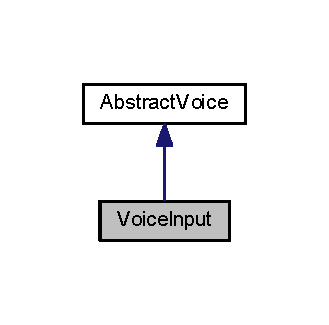
\includegraphics[width=178pt]{class_voice_input__inherit__graph}
\end{center}
\end{figure}


\-Collaboration diagram for \-Voice\-Input\-:\nopagebreak
\begin{figure}[H]
\begin{center}
\leavevmode
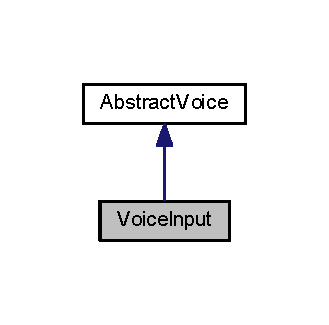
\includegraphics[width=293pt]{class_voice_input__coll__graph}
\end{center}
\end{figure}
\subsection*{\-Public \-Slots}
\begin{DoxyCompactItemize}
\item 
virtual void \hyperlink{class_voice_input_a99193e448e78f1bd10219bfb482d13ba}{start} ()
\begin{DoxyCompactList}\small\item\em \-Implemented virtual start method from \hyperlink{class_abstract_voice}{\-Abstract\-Voice}. \end{DoxyCompactList}\item 
virtual void \hyperlink{class_voice_input_aacdc744a4d9b156d79d05c7ea9361576}{stop} ()
\begin{DoxyCompactList}\small\item\em \-Implemented virtual stop method from \hyperlink{class_abstract_voice}{\-Abstract\-Voice}. \end{DoxyCompactList}\end{DoxyCompactItemize}
\subsection*{\-Public \-Member \-Functions}
\begin{DoxyCompactItemize}
\item 
\hyperlink{class_voice_input_a57880cf450adb3749b952de271b8261f}{\-Voice\-Input} (\-Q\-Host\-Address address)
\begin{DoxyCompactList}\small\item\em \-Creates our \-Audio\-Device object and buffer used. \end{DoxyCompactList}\item 
\hyperlink{class_voice_input_a9ebb274fbb6075af8feb26f2cd3b6e93}{$\sim$\-Voice\-Input} ()
\begin{DoxyCompactList}\small\item\em \-Default destructor. \end{DoxyCompactList}\end{DoxyCompactItemize}
\subsection*{\-Public \-Attributes}
\begin{DoxyCompactItemize}
\item 
\hyperlink{class_sound_sender}{\-Sound\-Sender} \hyperlink{class_voice_input_a40ab6705a21bcbaae15e9a673f6eee53}{send}
\end{DoxyCompactItemize}
\subsection*{\-Private \-Slots}
\begin{DoxyCompactItemize}
\item 
virtual void \hyperlink{class_voice_input_a2481e823c393974288383a7f470054ad}{audio\-State} (\-Q\-Audio\-::\-State)
\begin{DoxyCompactList}\small\item\em \-Implemented virtual slot from \hyperlink{class_abstract_voice}{\-Abstract\-Voice}. \end{DoxyCompactList}\item 
void \hyperlink{class_voice_input_a6f48cb2d0fb8239c284545fda2c099bb}{mute\-Mic} (bool)
\begin{DoxyCompactList}\small\item\em \-Mutes the \-Mic of sound until toggled via this method. \end{DoxyCompactList}\end{DoxyCompactItemize}
\subsection*{\-Private \-Attributes}
\begin{DoxyCompactItemize}
\item 
\-Q\-Audio\-Input $\ast$ \hyperlink{class_voice_input_a8e65f3f1987db8213d8b10f1bcaaab00}{m\-\_\-audio\-In}
\begin{DoxyCompactList}\small\item\em \-The \-Input device object. \end{DoxyCompactList}\end{DoxyCompactItemize}


\subsection{\-Detailed \-Description}
\-Captures audio data and puts it in a buffer for sending down the network. 

\-This class captures data from the systems native input device and adds it to a buffer to be sent down the network. \-It is assumed that the format of this audio data is the same as represented by this classes superclass \hyperlink{class_abstract_voice}{\-Abstract\-Voice}. 

\subsection{\-Constructor \& \-Destructor \-Documentation}
\hypertarget{class_voice_input_a57880cf450adb3749b952de271b8261f}{
\index{\-Voice\-Input@{\-Voice\-Input}!\-Voice\-Input@{\-Voice\-Input}}
\index{\-Voice\-Input@{\-Voice\-Input}!VoiceInput@{\-Voice\-Input}}
\subsubsection[{\-Voice\-Input}]{\setlength{\rightskip}{0pt plus 5cm}\-Voice\-Input\-::\-Voice\-Input (
\begin{DoxyParamCaption}
\item[{\-Q\-Host\-Address}]{address}
\end{DoxyParamCaption}
)\hspace{0.3cm}{\ttfamily  \mbox{[}explicit\mbox{]}}}}
\label{class_voice_input_a57880cf450adb3749b952de271b8261f}


\-Creates our \-Audio\-Device object and buffer used. 


\begin{DoxyParams}{\-Parameters}
{\em address} & \-The address to send captured data. \\
\hline
\end{DoxyParams}
\hypertarget{class_voice_input_a9ebb274fbb6075af8feb26f2cd3b6e93}{
\index{\-Voice\-Input@{\-Voice\-Input}!$\sim$\-Voice\-Input@{$\sim$\-Voice\-Input}}
\index{$\sim$\-Voice\-Input@{$\sim$\-Voice\-Input}!VoiceInput@{\-Voice\-Input}}
\subsubsection[{$\sim$\-Voice\-Input}]{\setlength{\rightskip}{0pt plus 5cm}\-Voice\-Input\-::$\sim$\-Voice\-Input (
\begin{DoxyParamCaption}
{}
\end{DoxyParamCaption}
)}}
\label{class_voice_input_a9ebb274fbb6075af8feb26f2cd3b6e93}


\-Default destructor. 



\subsection{\-Member \-Function \-Documentation}
\hypertarget{class_voice_input_a2481e823c393974288383a7f470054ad}{
\index{\-Voice\-Input@{\-Voice\-Input}!audio\-State@{audio\-State}}
\index{audio\-State@{audio\-State}!VoiceInput@{\-Voice\-Input}}
\subsubsection[{audio\-State}]{\setlength{\rightskip}{0pt plus 5cm}void \-Voice\-Input\-::audio\-State (
\begin{DoxyParamCaption}
\item[{\-Q\-Audio\-::\-State}]{state}
\end{DoxyParamCaption}
)\hspace{0.3cm}{\ttfamily  \mbox{[}private, virtual, slot\mbox{]}}}}
\label{class_voice_input_a2481e823c393974288383a7f470054ad}


\-Implemented virtual slot from \hyperlink{class_abstract_voice}{\-Abstract\-Voice}. 

\-This is connected to changes in our \-Audio\-Output object. 

\-Implements \hyperlink{class_abstract_voice_a4c8d0cafd33f068899f8700f00e93347}{\-Abstract\-Voice}.

\hypertarget{class_voice_input_a6f48cb2d0fb8239c284545fda2c099bb}{
\index{\-Voice\-Input@{\-Voice\-Input}!mute\-Mic@{mute\-Mic}}
\index{mute\-Mic@{mute\-Mic}!VoiceInput@{\-Voice\-Input}}
\subsubsection[{mute\-Mic}]{\setlength{\rightskip}{0pt plus 5cm}void \-Voice\-Input\-::mute\-Mic (
\begin{DoxyParamCaption}
\item[{bool}]{toggle}
\end{DoxyParamCaption}
)\hspace{0.3cm}{\ttfamily  \mbox{[}private, slot\mbox{]}}}}
\label{class_voice_input_a6f48cb2d0fb8239c284545fda2c099bb}


\-Mutes the \-Mic of sound until toggled via this method. 

\hypertarget{class_voice_input_a99193e448e78f1bd10219bfb482d13ba}{
\index{\-Voice\-Input@{\-Voice\-Input}!start@{start}}
\index{start@{start}!VoiceInput@{\-Voice\-Input}}
\subsubsection[{start}]{\setlength{\rightskip}{0pt plus 5cm}void \-Voice\-Input\-::start (
\begin{DoxyParamCaption}
{}
\end{DoxyParamCaption}
)\hspace{0.3cm}{\ttfamily  \mbox{[}virtual, slot\mbox{]}}}}
\label{class_voice_input_a99193e448e78f1bd10219bfb482d13ba}


\-Implemented virtual start method from \hyperlink{class_abstract_voice}{\-Abstract\-Voice}. 

\-This method starts recording and filling the network buffer. 

\-Implements \hyperlink{class_abstract_voice_a5e6f942915e9ef55babd7070225266ce}{\-Abstract\-Voice}.

\hypertarget{class_voice_input_aacdc744a4d9b156d79d05c7ea9361576}{
\index{\-Voice\-Input@{\-Voice\-Input}!stop@{stop}}
\index{stop@{stop}!VoiceInput@{\-Voice\-Input}}
\subsubsection[{stop}]{\setlength{\rightskip}{0pt plus 5cm}void \-Voice\-Input\-::stop (
\begin{DoxyParamCaption}
{}
\end{DoxyParamCaption}
)\hspace{0.3cm}{\ttfamily  \mbox{[}virtual, slot\mbox{]}}}}
\label{class_voice_input_aacdc744a4d9b156d79d05c7ea9361576}


\-Implemented virtual stop method from \hyperlink{class_abstract_voice}{\-Abstract\-Voice}. 

\-This method stops recording. 

\-Implements \hyperlink{class_abstract_voice_aae2a6c918a63938881faefd9909508a0}{\-Abstract\-Voice}.



\subsection{\-Member \-Data \-Documentation}
\hypertarget{class_voice_input_a8e65f3f1987db8213d8b10f1bcaaab00}{
\index{\-Voice\-Input@{\-Voice\-Input}!m\-\_\-audio\-In@{m\-\_\-audio\-In}}
\index{m\-\_\-audio\-In@{m\-\_\-audio\-In}!VoiceInput@{\-Voice\-Input}}
\subsubsection[{m\-\_\-audio\-In}]{\setlength{\rightskip}{0pt plus 5cm}\-Q\-Audio\-Input$\ast$ {\bf \-Voice\-Input\-::m\-\_\-audio\-In}\hspace{0.3cm}{\ttfamily  \mbox{[}private\mbox{]}}}}
\label{class_voice_input_a8e65f3f1987db8213d8b10f1bcaaab00}


\-The \-Input device object. 

\hypertarget{class_voice_input_a40ab6705a21bcbaae15e9a673f6eee53}{
\index{\-Voice\-Input@{\-Voice\-Input}!send@{send}}
\index{send@{send}!VoiceInput@{\-Voice\-Input}}
\subsubsection[{send}]{\setlength{\rightskip}{0pt plus 5cm}{\bf \-Sound\-Sender} {\bf \-Voice\-Input\-::send}}}
\label{class_voice_input_a40ab6705a21bcbaae15e9a673f6eee53}


\-The documentation for this class was generated from the following files\-:\begin{DoxyCompactItemize}
\item 
\hyperlink{voiceinput_8h}{voiceinput.\-h}\item 
\hyperlink{voiceinput_8cpp}{voiceinput.\-cpp}\end{DoxyCompactItemize}

\hypertarget{class_voice_output}{
\section{\-Voice\-Output \-Class \-Reference}
\label{class_voice_output}\index{\-Voice\-Output@{\-Voice\-Output}}
}


\-Receives audio data and plays it using the systems default output device.  




{\ttfamily \#include $<$voiceoutput.\-h$>$}



\-Inheritance diagram for \-Voice\-Output\-:\nopagebreak
\begin{figure}[H]
\begin{center}
\leavevmode
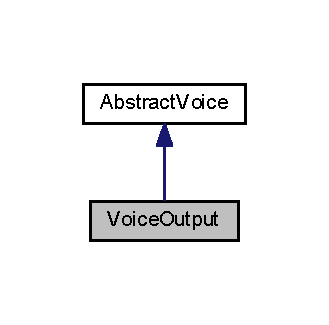
\includegraphics[width=158pt]{class_voice_output__inherit__graph}
\end{center}
\end{figure}


\-Collaboration diagram for \-Voice\-Output\-:\nopagebreak
\begin{figure}[H]
\begin{center}
\leavevmode
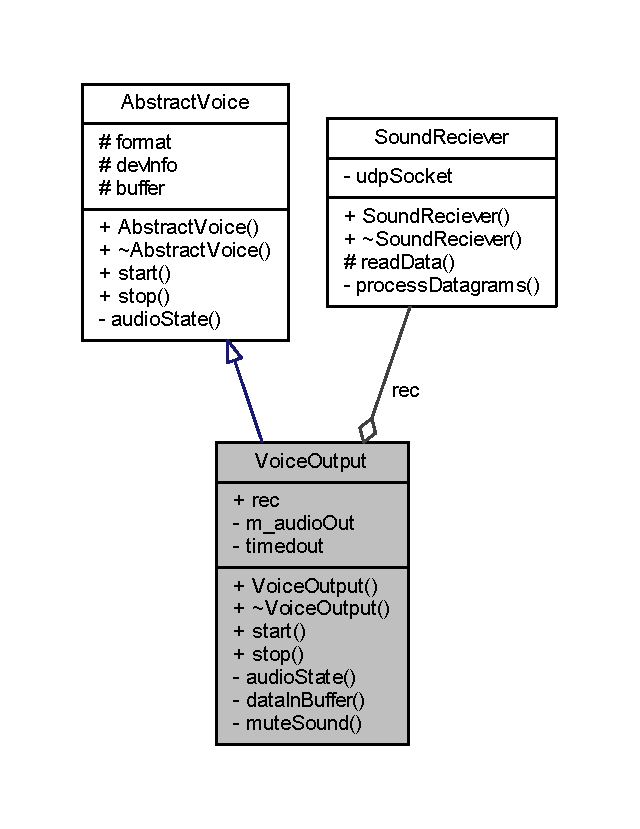
\includegraphics[width=158pt]{class_voice_output__coll__graph}
\end{center}
\end{figure}
\subsection*{\-Public \-Slots}
\begin{DoxyCompactItemize}
\item 
virtual void \hyperlink{class_voice_output_ab73d7fc81805b8ba0d457db2fcf29ac4}{start} ()
\begin{DoxyCompactList}\small\item\em \-Implemented virtual start method from \hyperlink{class_abstract_voice}{\-Abstract\-Voice}. \end{DoxyCompactList}\item 
virtual void \hyperlink{class_voice_output_ad86ffb5732b221da79f5bfba04e7a35a}{stop} ()
\begin{DoxyCompactList}\small\item\em \-Implemented virtual stop method from \hyperlink{class_abstract_voice}{\-Abstract\-Voice}. \end{DoxyCompactList}\end{DoxyCompactItemize}
\subsection*{\-Public \-Member \-Functions}
\begin{DoxyCompactItemize}
\item 
\hyperlink{class_voice_output_a82e8a7dc2eb2de4520e1fbe7e0f71e30}{\-Voice\-Output} (\hyperlink{class_abstract_voice}{\-Abstract\-Voice} $\ast$parent=0)
\begin{DoxyCompactList}\small\item\em \-Default constructor. \end{DoxyCompactList}\item 
\hypertarget{class_voice_output_ab483f1f9a463ed3cd3e5fb265147e51e}{
\hyperlink{class_voice_output_ab483f1f9a463ed3cd3e5fb265147e51e}{$\sim$\-Voice\-Output} ()}
\label{class_voice_output_ab483f1f9a463ed3cd3e5fb265147e51e}

\begin{DoxyCompactList}\small\item\em \-Default destructor. \end{DoxyCompactList}\end{DoxyCompactItemize}


\subsection{\-Detailed \-Description}
\-Receives audio data and plays it using the systems default output device. 

\-This class receives data from a buffer of audio data and subsequently plays it. \-It is assumed that the format of this audio data is the same as represented by this classes superclass \hyperlink{class_abstract_voice}{\-Abstract\-Voice}. 

\subsection{\-Constructor \& \-Destructor \-Documentation}
\hypertarget{class_voice_output_a82e8a7dc2eb2de4520e1fbe7e0f71e30}{
\index{\-Voice\-Output@{\-Voice\-Output}!\-Voice\-Output@{\-Voice\-Output}}
\index{\-Voice\-Output@{\-Voice\-Output}!VoiceOutput@{\-Voice\-Output}}
\subsubsection[{\-Voice\-Output}]{\setlength{\rightskip}{0pt plus 5cm}\-Voice\-Output\-::\-Voice\-Output (
\begin{DoxyParamCaption}
\item[{{\bf \-Abstract\-Voice} $\ast$}]{parent = {\ttfamily 0}}
\end{DoxyParamCaption}
)\hspace{0.3cm}{\ttfamily  \mbox{[}explicit\mbox{]}}}}
\label{class_voice_output_a82e8a7dc2eb2de4520e1fbe7e0f71e30}


\-Default constructor. 

\-Creates our \-Audio\-Device object and buffer used. 
\begin{DoxyParams}{\-Parameters}
{\em parent} & \-The owner of this object. \\
\hline
\end{DoxyParams}


\subsection{\-Member \-Function \-Documentation}
\hypertarget{class_voice_output_ab73d7fc81805b8ba0d457db2fcf29ac4}{
\index{\-Voice\-Output@{\-Voice\-Output}!start@{start}}
\index{start@{start}!VoiceOutput@{\-Voice\-Output}}
\subsubsection[{start}]{\setlength{\rightskip}{0pt plus 5cm}void \-Voice\-Output\-::start (
\begin{DoxyParamCaption}
{}
\end{DoxyParamCaption}
)\hspace{0.3cm}{\ttfamily  \mbox{[}virtual, slot\mbox{]}}}}
\label{class_voice_output_ab73d7fc81805b8ba0d457db2fcf29ac4}


\-Implemented virtual start method from \hyperlink{class_abstract_voice}{\-Abstract\-Voice}. 

\-This method starts listening trying to get data from the buffer for playback. 

\-Implements \hyperlink{class_abstract_voice_a5e6f942915e9ef55babd7070225266ce}{\-Abstract\-Voice}.

\hypertarget{class_voice_output_ad86ffb5732b221da79f5bfba04e7a35a}{
\index{\-Voice\-Output@{\-Voice\-Output}!stop@{stop}}
\index{stop@{stop}!VoiceOutput@{\-Voice\-Output}}
\subsubsection[{stop}]{\setlength{\rightskip}{0pt plus 5cm}void \-Voice\-Output\-::stop (
\begin{DoxyParamCaption}
{}
\end{DoxyParamCaption}
)\hspace{0.3cm}{\ttfamily  \mbox{[}virtual, slot\mbox{]}}}}
\label{class_voice_output_ad86ffb5732b221da79f5bfba04e7a35a}


\-Implemented virtual stop method from \hyperlink{class_abstract_voice}{\-Abstract\-Voice}. 

\-This method stops listening. 

\-Implements \hyperlink{class_abstract_voice_aae2a6c918a63938881faefd9909508a0}{\-Abstract\-Voice}.



\-The documentation for this class was generated from the following files\-:\begin{DoxyCompactItemize}
\item 
voiceoutput.\-h\item 
voiceoutput.\-cpp\end{DoxyCompactItemize}

\printindex
\end{document}
